%\documentclass[handout]{beamer}
\documentclass{beamer}

\mode<presentation>
{
%\usetheme{Singapore}
%\usetheme{Warsaw}
\usetheme{Malmoe}
\useinnertheme{circles}
\useoutertheme{infolines}
% \useinnertheme{rounded}

\setbeamercovered{transparent}
}

\usepackage[english]{babel}
\usepackage[latin1]{inputenc}
\usepackage{bm,textpos,alltt,listings,multirow,ulem,minted}
\usepackage{JedMacros}

% font definitions, try \usepackage{ae} instead of the following
% three lines if you don't like this look
\usepackage{mathptmx}
\usepackage[scaled=.90]{helvet}
\usepackage{courier}
\usepackage[T1]{fontenc}
\usepackage{tikz}
\usetikzlibrary[shapes.arrows,arrows,shapes.misc]

% \usepackage{pgfpages}
% \pgfpagesuselayout{4 on 1}[letterpaper,landscape,border shrink=5mm]

% Macros for the p-Bratu revision numbers
\def\Rbasic{0}
\def\Rrlap{1}
\def\Rrbratu{2}
\def\Rrpbratu{3}
\def\Rassemblebratu{4}
\def\Rassemblepicard{5}
\def\Rmyprealloc{6}
\def\Rnewtoncrash{7}
\def\Rnewtonbug{8}
\def\Rnewtonfix{9}

\title[PETSc]{The Portable Extensible Toolkit for Scientific computing}

\author{Barry Smith}


% - Use the \inst command only if there are several affiliations.
% - Keep it simple, no one is interested in your street address.
\institute[ANL]{Mathematics and Computer Science Division, Argonne National Laboratory}

\date{ATPESC 2013-08-02}


% This is only inserted into the PDF information catalog. Can be left
% out.
\subject{Talks}



% If you have a file called "university-logo-filename.xxx", where xxx
% is a graphic format that can be processed by latex or pdflatex,
% resp., then you can add a logo as follows:

% \pgfdeclareimage[height=0.5cm]{university-logo}{university-logo-filename}
% \logo{\pgfuseimage{university-logo}}



% Delete this, if you do not want the table of contents to pop up at
% the beginning of each subsection:
\AtBeginSubsection[]
{
 \begin{frame}<beamer>
 \frametitle{Outline}
 \tableofcontents[currentsection,currentsubsection]
 \end{frame}
}

\AtBeginSection[]{
\begin{frame}<beamer>
  \frametitle{Outline}
  \tableofcontents[currentsection]
\end{frame}
}

% If you wish to uncover everything in a step-wise fashion, uncomment
% the following command:

%\beamerdefaultoverlayspecification{<+->}

\begin{document}
\lstset{language=C}

\begin{frame}
\titlepage
Thanks to Jed Brown and Matt Knepley for the slides
\end{frame}

\begin{frame}
\frametitle{Outline}
\tableofcontents
% You might wish to add the option [pausesections]
\end{frame}
\begin{frame}{Follow Up; Getting Help}
  \begin{itemize}
    \item http://www.mcs.anl.gov/petsc
    \item Configuration issues, private: \url{petsc-maint@mcs.anl.gov}
    \item Public questions: \url{petsc-users@mcs.anl.gov}
    \item Today, speak with
    \begin{itemize}
      \item me
      \item Satish Balay
      \item Jed Brown
      \item Lois McInnes
    \end{itemize}
  \end{itemize}
\end{frame}


\section{Introduction}
\newcommand\ganttline[4]{% line, tag, start end
   \node at (0,#1*0.4+.1) [anchor=base east] {#2};
   \fill[blue] (#3/\xtick-1991/\xtick,#1*0.4-.1) rectangle (#4/\xtick-1991/\xtick,#1*0.4+.1);}
\newcommand\ganttlabel[6]{% year, label, color, yloc, anchor
  \node[#3] at (#1/\xtick+#6/\xtick-1991/\xtick,#4) [anchor=#5] {#2};
  \fill[#3] (#1/\xtick-1991/\xtick,1/2-.1) rectangle (#1/\xtick-1991/\xtick+0.04,12/2+.1);}

%\begin{frame}{Timeline}
\frame{
\begin{figure}[htbp]
\def\present{2013.5}
\def\xtick{2.2}
\begin{tikzpicture}[y=-1cm]
   %\draw[help lines] (0.5,5) grid (8,0.5);
   \ganttlabel{1991}{1991}{red}{6.2}{north}{0}
   \ganttlabel{1995}{1995}{red}{6.2}{north}{0}
   \ganttlabel{2000}{2000}{red}{6.2}{north}{0}
   \ganttlabel{2005}{2005}{red}{6.2}{north}{0}
   \ganttlabel{2010}{2010}{red}{6.2}{north}{0}
   \ganttlabel{1992}{PETSc-1}{green!70!black}{0}{center}{0}
   \ganttlabel{1994.4}{MPI-1}{magenta!70!black}{-.5}{center}{0}
   \ganttlabel{1997.6}{MPI-2}{magenta!70!black}{-.5}{center}{0}
   \ganttlabel{1995.5}{PETSc-2}{green!70!black}{0}{center}{0}
   \ganttlabel{2008.9}{PETSc-3}{green!70!black}{0}{center}{0}
   \ganttline{1}{Barry}{1991}{\present}
   \ganttline{2}{Bill}{1991}{1996}
   \ganttline{3}{Lois}{1993}{2001}
   \ganttline{4}{Satish}{1997}{\present}
   \ganttline{5}{Dinesh}{1998}{2005.5}
   \ganttline{6}{Hong}{2001}{\present}
   \ganttline{7}{Kris}{2001}{2006}
   \ganttline{8}{Matt}{2001.5}{\present}
   \ganttline{9}{Victor}{2003}{2006.9}
   \ganttline{9}{}{2007.3}{2007.5}
   \ganttline{9}{}{2008.5}{2008.7}
   \ganttline{10}{Dmitry}{2005.6}{\present}
   \ganttline{11}{Lisandro}{2006.9}{\present}
   \ganttline{12}{Jed}{2009}{\present}
   \ganttline{13}{Shri}{2009.8}{\present}
   \ganttline{14}{Peter}{2011.6}{\present}
\end{tikzpicture}
\end{figure}
}
%\end{frame}

\begin{frame}{Commits to the PETSc Repository}

\begin{center}
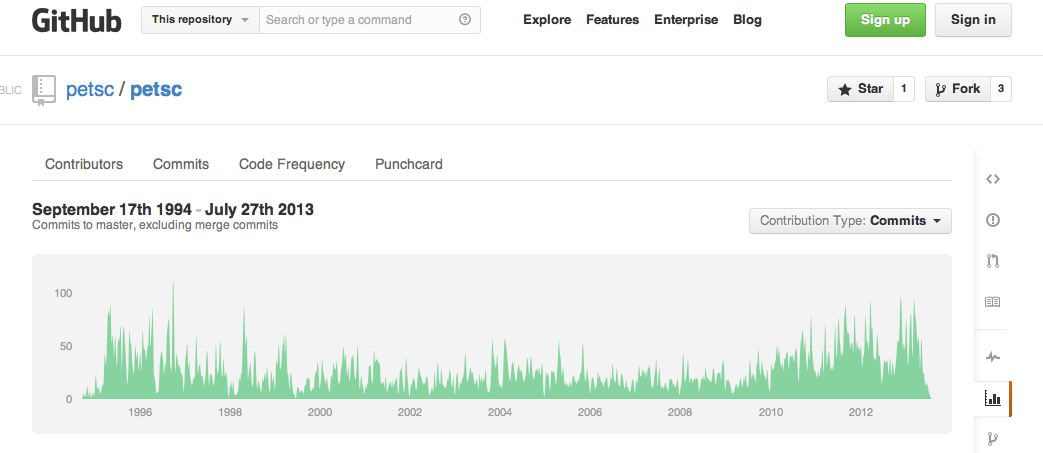
\includegraphics[width=5.0in]{figures/PETSc/Commits}
\end{center}

\end{frame}

\begin{frame}{{\bf Portable} Extensible Toolkit for Scientific computing}
%TODO: big-iron image
\begin{itemize}
  \item Architecture
    \begin{itemize}
    \item tightly coupled (e.g. XT5, BG/P, Earth Simulator)
    \item loosely coupled such as network of workstations
    \end{itemize}
  \item Operating systems (Linux, Mac, Windows, BSD, proprietary Unix)
  \item Any compiler
  \item Real/complex, single/double precision, 32/64-bit int
  \item Usable from C, C++, Fortran 77/90, and Python
  \item Free to everyone (BSD-style license), open development
  \item 500B unknowns, 75\% weak scalability on Jaguar (225k cores) \\
    and Jugene (295k cores)
  \item Same code runs performantly on a laptop
  \item<2> \alert{\tikz[baseline] \node [cross out,draw=black,line width=1,anchor=text] {No}; iPhone support}
\end{itemize}
\end{frame}

\begin{frame}{Portable {\bf Extensible} Toolkit for Scientific computing}
\begin{block}{Philosophy: Everything has a plugin architecture}
\begin{itemize}
  \item Vectors, Matrices, Coloring/ordering/partitioning algorithms
  \item Preconditioners, Krylov accelerators
  \item Nonlinear solvers, Time integrators
  \item Spatial discretizations/topology$^*$
\end{itemize}
\end{block}
\begin{example}
	Vendor supplies matrix format and associated preconditioner, distributes
	compiled shared library.  Application user loads plugin at runtime, no source
	code in sight.
\end{example}
\end{frame}

\begin{frame}{Portable Extensible {\bf Toolkit} for Scientific computing}
Algorithms, (parallel) debugging aids, low-overhead profiling
\begin{block}{Composability}
Try new algorithms by choosing from product space and composing
existing algorithms (multilevel, domain decomposition, splitting).
\end{block}
\begin{block}{Experimentation}
\begin{itemize}
  \item It is not possible to pick the solver \emph{a priori}. \\
  What will deliver best/competitive performance for a given physics, discretization, architecture, and problem size?
  \item PETSc's response: expose an algebra of composition so new solvers can be created at runtime.
  \item Important to keep solvers decoupled from physics and discretization because we also experiment with those. 
\end{itemize}
\end{block}
\end{frame}

\begin{frame}{Portable Extensible Toolkit for {\bf Scientific computing}}
  \begin{itemize}
  \item Computational Scientists
    \begin{itemize}
    \item PyLith (CIG), Underworld (Monash), Magma Dynamics (LDEO, Columbia), PFLOTRAN (DOE), SHARP/UNIC (DOE)
    \end{itemize}
  \item Algorithm Developers (iterative methods and preconditioning)
  \item Package Developers
    \begin{itemize}
    \item SLEPc, TAO, Deal.II, Libmesh, FEniCS, PETSc-FEM, MagPar, OOFEM, FreeCFD, OpenFVM
    \end{itemize}
  \item Funding
    \begin{itemize}\item Department of Energy
      \begin{itemize}\item SciDAC, ASCR ISICLES, MICS Program, INL Reactor Program
      \end{itemize}
    \item National Science Foundation
      \begin{itemize}\item CIG, CISE, Multidisciplinary Challenge Program
      \end{itemize}
    \end{itemize}
  \item Hundreds of tutorial-style examples
  \item Hyperlinked manual, examples, and manual pages for all routines
  \item Support from \url{petsc-maint@mcs.anl.gov}
  %\item Mailing list \url{petsc-users@mcs.anl.gov}
\end{itemize}
\end{frame}

\frame{
\frametitle{The Role of PETSc}

\vspace*{\fill}
\begin{minipage}{\linewidth}
\begin{quote}
\Large Developing parallel, nontrivial PDE solvers that deliver high performance is still difficult and requires
months (or even years) of concentrated effort.

\medskip

PETSc is a toolkit that can ease these difficulties and reduce the development time, but it is not a black-box PDE
solver, nor a \blue{silver bullet}.
\end{quote}
\qquad --- Barry Smith
\end{minipage}
\vspace*{\fill}\vspace*{\fill}
}



\begin{frame}{Better To Use than PETSc}
 Use the package with the highest level of abstraction that uses PETSc

    \begin{itemize}
    \item Eigenvalues - SLEPc,
    \item Optimizationation (with PDE constraints) - TAO
    \item Finite Elements -  Deal.II, Libmesh, FEniCS, PETSc-FEM,  OOFEM, 
    \item Finite Elements and Multiphysics - MOOSE 
    \item Finite Volumes -  FreeCFD, OpenFVM
    \item Wave Propagation - PyClaw
    \item Micromagnetics - MagPar
    \end{itemize}
\end{frame}





\begin{frame}{Advice from Bill Gropp}
  \begin{quote}\large
    You want to think about how you decompose your data structures, how
    you think about them globally.  [...]  If you were building a house,
    you'd start with a set of blueprints that give you a picture of what
    the whole house looks like.  You wouldn't start with a bunch of
    tiles and say. ``Well I'll put this tile down on the ground, and
    then I'll find a tile to go next to it.''  But all too many people
    try to build their parallel programs by creating the smallest
    possible tiles and then trying to have the structure of their code
    emerge from the chaos of all these little pieces.  You have to have
    an organizing principle if you're going to survive making your code
    parallel.
  \end{quote}
  {\small \centering (\url{http://www.rce-cast.com/Podcast/rce-28-mpich2.html})}
\end{frame}


\begin{frame}{PETSc Structure}

\begin{center}
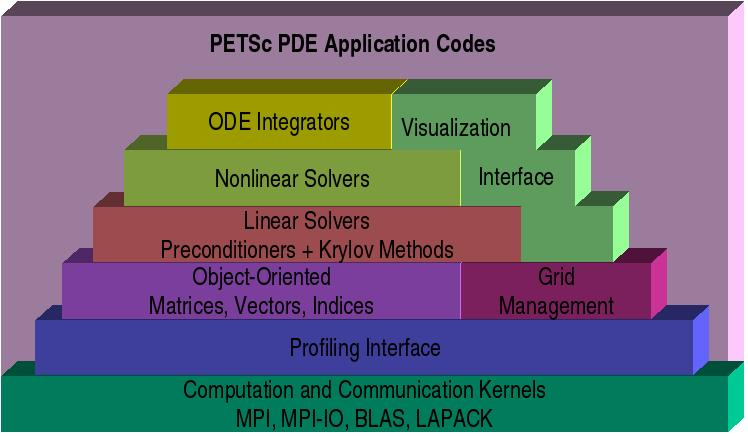
\includegraphics[width=5.0in]{figures/PETSc/PETScPyramid}
\end{center}

\end{frame}


\section{Objects - Building Blocks of the Code}


\begin{frame}{MPI communicators}
  \begin{itemize}
  \item Opaque object, defines process group and synchronization channel
  \item PETSc objects need an \code{MPI\_Comm} in their constructor
    \begin{itemize}
    \item \code{PETSC\_COMM\_SELF} for serial objects
    \item \code{PETSC\_COMM\_WORLD} common, but \emph{not} required
    \end{itemize}
  \item Can split communicators, spawn processes on new communicators, etc
  \item Operations are one of
    \begin{itemize}
    \item Not Collective: \code{VecGetLocalSize(), MatSetValues()}
    \item Logically Collective: \code{KSPSetType(), PCMGSetCycleType()}
      \begin{itemize}
      \item checked when running in debug mode
      \end{itemize}
    \item Neighbor-wise Collective: \code{VecScatterBegin(), MatMult()}
      \begin{itemize}
      \item Point-to-point communication between two processes
      \item Neighbor collectives in upcoming MPI-3
      \end{itemize}
    \item Collective: \code{VecNorm(), MatAssemblyBegin(), KSPCreate()}
      \begin{itemize}
      \item Global communication, synchronous
      \item Non-blocking collectives in upcoming MPI-3
      \end{itemize}
    \end{itemize}
  \item Deadlock if some process doesn't participate (\eg wrong order)
  \end{itemize}
\end{frame}



\subsection{Options Database}
\begin{frame}[fragile]{Objects}
  % \begin{lstlisting}
  %   Mat A;
  %   PetscInt m,n,M,N;
  %   MatCreate(comm,&A);
  %   MatSetSizes(A,m,n,M,N);      /* or PETSC_DECIDE */ 
  %   MatSetOptionsPrefix(A,"foo_");
  %   MatSetFromOptions(A);
  %   /* Use A */
  %   MatView(A,PETSC_VIEWER_DRAW_WORLD);
  %   MatDestroy(A);
  % \end{lstlisting}
  \begin{minted}{c}
    Mat A;
    PetscInt m,n,M,N;
    MatCreate(comm,&A);
    MatSetSizes(A,m,n,M,N);      /* or PETSC_DECIDE */ 
    MatSetOptionsPrefix(A,"foo_");
    MatSetFromOptions(A);
    /* Use A */
    MatView(A,PETSC_VIEWER_DRAW_WORLD);
    MatDestroy(A);
  \end{minted}
  \begin{itemize}
  \item \code{Mat} is an opaque object (pointer to incomplete type)
    \oneitem{Assignment, comparison, etc, are cheap}
  \item What's up with this ``Options'' stuff?
    \begin{itemize}
    \item Allows the type to be determined at runtime: \code{-foo\_mat\_type sbaij}
    \item Inversion of Control similar to ``service locator'', \\
      related to ``dependency injection''
    \item Other options (performance and semantics) can be changed at
      runtime under \code{-foo\_mat\_}
    \end{itemize}
  \end{itemize}
\end{frame}

\begin{frame}{Basic {\kb PetscObject} Usage}

\vbox{Every object in PETSc supports a basic interface}

\begin{tabular}{|r|l|}
\hline
Function & Operation \\
\hline
{\kb Create()}               & create the object \\
{\kb Get/SetName()}          & name the object \\
{\kb Get/SetType()}          & set the implementation type \\
{\kb Get/SetOptionsPrefix()} & set the prefix for all options \\
{\kb SetFromOptions()}       & customize object from the command line \\
{\kb SetUp()}                & preform other initialization \\
{\kb View()}                 & view the object \\
{\kb Destroy()}              & cleanup object allocation \\
\hline
\end{tabular}

\vbox{Also, all objects support the {\kb -help} option.}

\end{frame}


\begin{frame}{Ways to set options}
  \begin{itemize}
  \item Command line
  \item Filename in the third argument of \code{PetscInitialize()}
  \item \code{$\sim$/.petscrc}
  \item \code{\$PWD/.petscrc}
  \item \code{\$PWD/petscrc}
  \item \code{PetscOptionsInsertFile()}
  \item \code{PetscOptionsInsertString()}
  \item \code{PETSC\_OPTIONS} environment variable
  \item command line option \code{-options\_file [file]}
  \end{itemize}
\end{frame}

\begin{frame}{Try it out}
  \shell{\small cd \$PETSC\_DIR/src/snes/examples/tutorials \&\& make ex5} \\
  \begin{itemize}
  \item \shell{./ex5 -da\_grid\_x 10 -da\_grid\_y 10 -par 6.7 \\
      -snes\_monitor -\{ksp,snes\}\_converged\_reason \\
      -snes\_view}
  \item \shell{./ex5 -da\_grid\_x 10 -da\_grid\_y 10 -par 6.7 \\
      -snes\_monitor -\{ksp,snes\}\_converged\_reason \\
      -snes\_view -mat\_view\_draw -draw\_pause 0.5}
  \item \shell{./ex5 -da\_grid\_x 10 -da\_grid\_y 10 -par 6.7 \\
      -snes\_monitor -\{ksp,snes\}\_converged\_reason \\
      -snes\_view -mat\_view\_draw -draw\_pause 0.5 \\
      -pc\_type lu -pc\_factor\_mat\_ordering\_type natural}
  \item Use \code{-help} to find other ordering types
\end{itemize}
\end{frame}

\begin{frame}[fragile]{Sample output}
\begin{Verbatim}[formatcom=\footnotesize]
  0 SNES Function norm 1.139460779565e+00 
  Linear solve converged due to CONVERGED_RTOL iterations 1
  1 SNES Function norm 4.144493702305e-02 
  Linear solve converged due to CONVERGED_RTOL iterations 1
  2 SNES Function norm 6.309075568032e-03 
  Linear solve converged due to CONVERGED_RTOL iterations 1
  3 SNES Function norm 3.359792279909e-04 
  Linear solve converged due to CONVERGED_RTOL iterations 1
  4 SNES Function norm 1.198827244256e-06 
  Linear solve converged due to CONVERGED_RTOL iterations 1
  5 SNES Function norm 1.545029314765e-11 
\end{Verbatim}
\vspace{-1em}
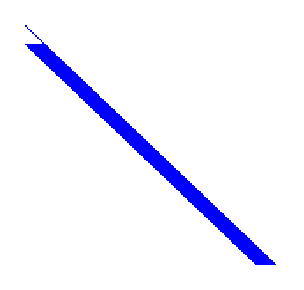
\includegraphics[width=0.5\textwidth]{figures/Ex5NaturalFill}
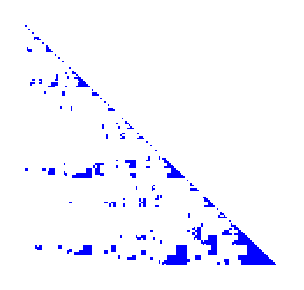
\includegraphics[width=0.5\textwidth]{figures/Ex5NDFill}
\end{frame}

\begin{frame}[fragile]{Sample output (SNES and KSP)}
\begin{Verbatim}[formatcom=\footnotesize]
SNES Object: 1 MPI processes
  type: ls
    line search variant: CUBIC
    alpha=1.000000000000e-04, maxstep=1.000000000000e+08, minlambda=1.000000000000e-12
    damping factor=1.000000000000e+00
  maximum iterations=50, maximum function evaluations=10000
  tolerances: relative=1e-08, absolute=1e-50, solution=1e-08
  total number of linear solver iterations=5
  total number of function evaluations=6
  KSP Object:   1 MPI processes
    type: gmres
      GMRES: restart=30, using Classical (unmodified) Gram-Schmidt Orthogonalization with no iterative refinement
      GMRES: happy breakdown tolerance 1e-30
    maximum iterations=10000, initial guess is zero
    tolerances:  relative=1e-05, absolute=1e-50, divergence=10000
    left preconditioning
    using PRECONDITIONED norm type for convergence test
\end{Verbatim}
\end{frame}
\begin{frame}[fragile]{Sample output (PC and Mat)}
\begin{Verbatim}[formatcom=\footnotesize]
  PC Object:   1 MPI processes
    type: lu
      LU: out-of-place factorization
      tolerance for zero pivot 2.22045e-14
      matrix ordering: nd
      factor fill ratio given 5, needed 2.95217
        Factored matrix follows:
          Matrix Object:           1 MPI processes
            type: seqaij
            rows=100, cols=100
            package used to perform factorization: petsc
            total: nonzeros=1358, allocated nonzeros=1358
            total number of mallocs used during MatSetValues calls =0
              not using I-node routines
    linear system matrix = precond matrix:
    Matrix Object:     1 MPI processes
      type: seqaij
      rows=100, cols=100
      total: nonzeros=460, allocated nonzeros=460
      total number of mallocs used during MatSetValues calls =0
        not using I-node routines
\end{Verbatim}
\end{frame}

\begin{frame}{In parallel}
  \begin{itemize}
  \item \shell{mpiexec -n 4 \\
      ./ex5 -da\_grid\_x 10 -da\_grid\_y 10 -par 6.7 \\
      -snes\_monitor -\{ksp,snes\}\_converged\_reason \\
      -snes\_view -sub\_pc\_type lu}
  \item How does the performance change as you
    \begin{itemize}
    \item vary the number of processes (up to 32 or 64)?
    \item increase the problem size?
    \item use an inexact subdomain solve?
    \item try an overlapping method: \code{-pc\_type asm -pc\_asm\_overlap 2}
    \item simulate a big machine: \code{-pc\_asm\_blocks 512}
    \item change the Krylov method: \code{-ksp\_type ibcgs}
    \item use algebraic multigrid: \code{-pc\_type hypre}
    \item use smoothed aggregation multigrid: \code{-pc\_type ml}
    \end{itemize}
  \end{itemize}
\end{frame}


\section[Core/Algorithms]{Core PETSc Components and Algorithms Primer}
\subsection{Time integration}
\begin{frame}[shrink=5]{IMEX time integration in PETSc}
  \begin{itemize}
  \item Additive Runge-Kutta IMEX methods
    \begin{gather*}
      G(t,x,\dot x) = F(t,x) \\
      J_\alpha = \alpha G_{\dot x} + G_x
    \end{gather*}
    \begin{itemize}
    \item User provides:
      \begin{itemize}
      \item \texttt{FormRHSFunction(ts,$t$,$x$,$F$,void *ctx);}
      \item \texttt{FormIFunction(ts,$t$,$x$,$\dot x$,$G$,void *ctx);}
      \item \texttt{FormIJacobian(ts,$t$,$x$,$\dot x$,$\alpha$,$J$,$J_{p}$,mstr,void *ctx);}
      \end{itemize}
    \item L-stable DIRK for stiff part $G$
    \item Choice of explicit method, \eg SSP
    \item Orders 2 through 5, embedded error estimates
    \item Dense output, hot starts for Newton
    \item More accurate methods if $G$ is linear, also Rosenbrock-W
    \item Can use preconditioner from classical ``semi-implicit'' methods
    \item Extensible adaptive controllers, can change order within a family
    \item Easy to register new methods: \code{TSARKIMEXRegister()}
    \end{itemize}
  \item Eliminate many interface quirks
  \item Single step interface so user can have own time loop
  \end{itemize}
\end{frame}

\frame{
\frametitle{Flow Control for a PETSc Application}

\begin{center}
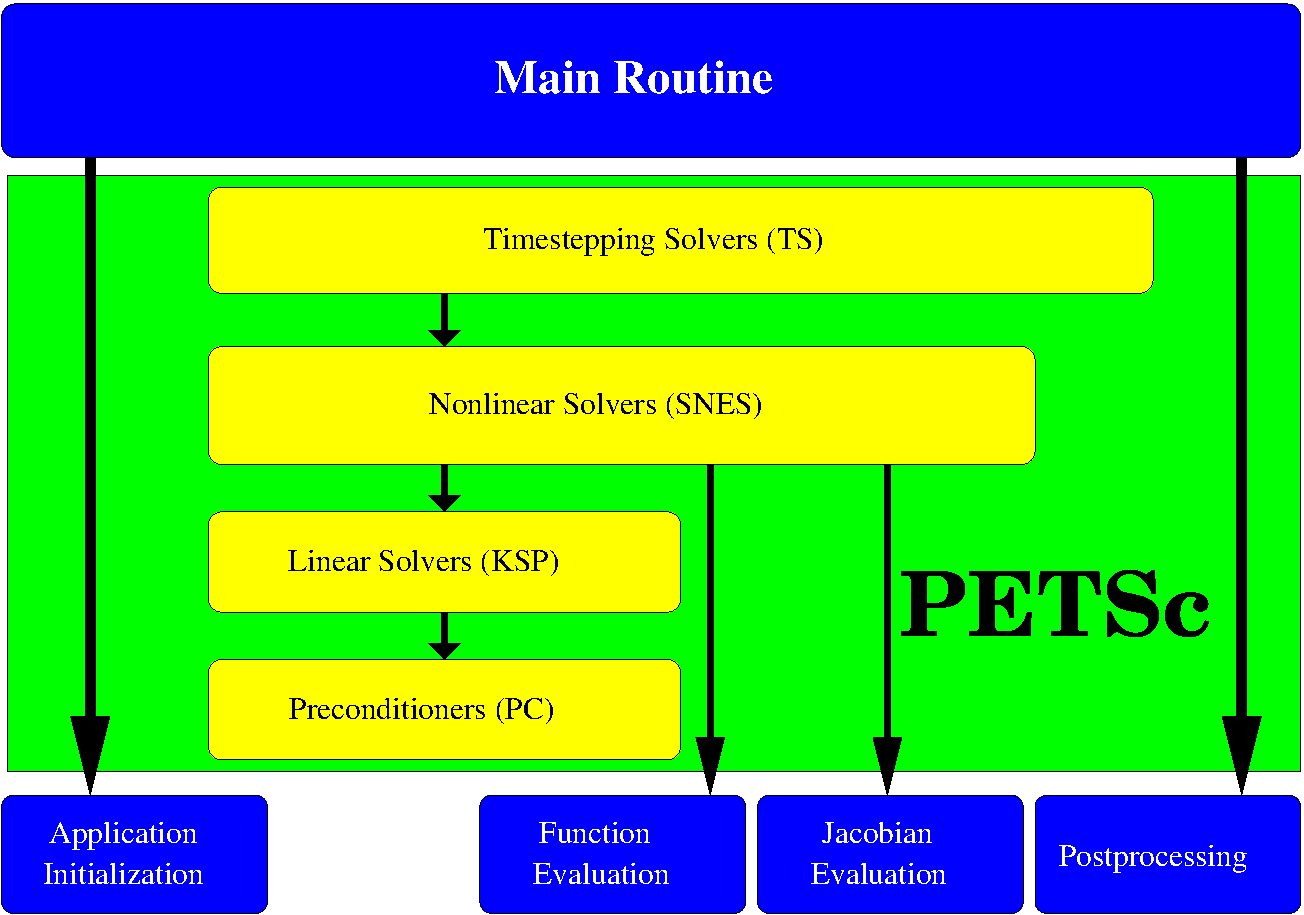
\includegraphics[width=4.0in]{figures/SNES/FlowControl}
\end{center}
}

\begin{frame}{Some TS methods}
  \begin{description}
  \item[TSSSPRK104] 10-stage, fourth order, low-storage, optimal explicit SSP Runge-Kutta $c_{\text{eff}} = 0.6$ (Ketcheson 2008)
  \item[TSARKIMEX2E] second order, one explicit and two implicit stages, $L$-stable, optimal (Constantinescu)
  \item[TSARKIMEX3] (and 4 and 5), $L$-stable (Kennedy and Carpenter, 2003)
  \item[TSROSWRA3PW] three stage, third order, for index-1 PDAE, $A$-stable, $R(\infty) = 0.73$, second order strongly $A$-stable embedded method (Rang and Angermann, 2005)
  \item[TSROSWRA34PW2] four stage, third order, $L$-stable, for index 1 PDAE, second order strongly $A$-stable embedded method (Rang and Angermann, 2005)
  \item[TSROSWLLSSP3P4S2C] four stage, third order, $L$-stable implicit, SSP explicit, $L$-stable embedded method (Constantinescu)
  \end{description}
\end{frame}

\begin{frame}{TS Examples}
  \begin{itemize}
  \item 1D nonlinear hyperbolic conservation laws
    \begin{itemize}
    \item \code{src/ts/examples/tutorials/ex9.c}
    \item {\footnotesize \code{./ex9 -da\_grid\_x 100 -initial 1 -physics shallow -limit minmod -ts\_ssp\_type rks2 -ts\_ssp\_nstages 8 -ts\_monitor\_solution}}
    \end{itemize}
  \item Stiff linear advection-reaction test problem
    \begin{itemize}
    \item \code{src/ts/examples/tutorials/ex22.c}
    \item {\footnotesize \code{./ex22 -da\_grid\_x 200 -ts\_monitor\_solution -ts\_type rosw -ts\_rosw\_type ra34pw2 -ts\_adapt\_monitor}}
    \end{itemize}
  \item 1D Brusselator (reaction-diffusion)
    \begin{itemize}
    \item \code{src/ts/examples/tutorials/ex25.c}
    \item {\footnotesize \code{./ex25 -da\_grid\_x 40 -ts\_monitor\_solution -ts\_type rosw -ts\_rosw\_type 2p -ts\_adapt\_monitor}}
    \end{itemize}
  \end{itemize}
\end{frame}


\subsection{Nonlinear solvers: SNES}
\begin{frame}{Newton iteration: workhorse of SNES}
  \begin{textblock}{3}(11,0)
    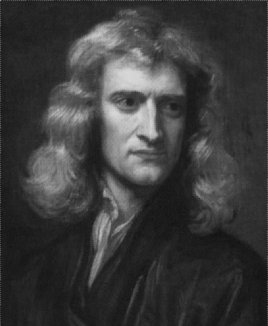
\includegraphics[width=\textwidth]{figures/Newton}
  \end{textblock}
  \begin{itemize}
  \item Standard form of a nonlinear system
    \[ F(u) = 0 \]
  \item Iteration
    \begin{align*}
      \text{Solve:} & \qquad J(u) w = -F(u) \\
      \text{Update:} & \qquad u^+ \gets u + w
    \end{align*}
    \item Quadratically convergent near a root: $\abs{u^{n+1}-u^*} \in \bigO\Big(\abs{u^n-u^*}^2\Big)$
    \item Picard is the same operation with a different $J(u)$
  \end{itemize}
  \begin{example}[Nonlinear Poisson]
    \begin{align*}
      F(u)=0 \quad &\sim\quad -\div\big[ (1+u^2) \nabla u \big] - f = 0 \\
      J(u)w \quad &\sim\quad  -\div\big[(1+u^2)\nabla w + 2uw\nabla u \Big]
    \end{align*}
  \end{example}
  % \begin{example}[$\pp$-Bratu]
  %   Suppose $F$ is a discretization of
  %   \[ -\nabla \cdot \big( \eta \nabla u \big) - \lambda e^u - f = 0 \]
  %   \[\eta(\gamma) = (\epsilon^2+\gamma)^{\frac{\pfrak-2}{2}}, \qquad\quad \gamma = \half \abs{\nabla u}^2. \]
  %   Then $J(u)w$ is a discretization of
  %   \[ -\nabla \cdot \big( \eta \nabla w + \eta' (\nabla u \cdot \nabla w)\nabla u \big) - \lambda e^{u} w . \]
  % \end{example}
\end{frame}


\begin{frame}
\frametitle{SNES Paradigm}

The SNES interface is based upon callback functions
\begin{itemize}
  \item \code{FormFunction()}, set by \code{SNESSetFunction()}

  \medskip

  \item \code{FormJacobian()}, set by \code{SNESSetJacobian()}
\end{itemize}

\bigskip

  When PETSc needs to evaluate the nonlinear residual $F(x)$,
\begin{itemize}
  \item Solver calls the {\bf user's} function

  \medskip

  \item User function gets application state through the {\kb ctx} variable
  \begin{itemize}
    \item PETSc \emph{never} sees application data
  \end{itemize}
\end{itemize}
\end{frame}

\begin{frame}{SNES Function}

The user provided function which calculates the nonlinear residual has signature
\begin{center}
  {\small \mint{c}|PetscErrorCode (*func)(SNES snes,Vec x,Vec r,void *ctx)|}
\end{center}
\begin{itemize}
  \item[{\kb x}:] The current solution
  \item[{\kb r}:] The residual
  \item[{\kb ctx}:] The user context passed to {\kb SNESSetFunction()}
  \begin{itemize}
    \item Use this to pass application information, e.g. physical constants
  \end{itemize}
\end{itemize}

\end{frame}

\begin{frame}[fragile]{SNES Jacobian}
The user provided function which calculates the Jacobian has signature
\begin{minted}{c}
PetscErrorCode (*func)(SNES snes,Vec x,Mat *J,Mat *M,
                       MatStructure *flag,void *ctx)
\end{minted}

\begin{itemize}
  \item[{\kb x}:] The current solution
  \item[{\kb J}:] The Jacobian
  \item[{\kb M}:] The Jacobian preconditioning matrix (possibly J itself)
  \item[{\kb ctx}:] The user context passed to {\kb SNESSetFunction()}
  \begin{itemize}
    \item Use this to pass application information, e.g. physical constants
  \end{itemize}

  \item Possible {\kb MatStructure} values are:
  \begin{itemize}
    \item SAME\_NONZERO\_PATTERN
    \item DIFFERENT\_NONZERO\_PATTERN
  \end{itemize}
\end{itemize}

Alternatively, you can use
\begin{itemize}
  \item a builtin sparse finite difference approximation (``coloring'')
  \item automatic differentiation (ADIC/ADIFOR)
\end{itemize}

\end{frame}



\subsection{Linear Algebra background/theory}
\begin{frame}{Matrices}
  \begin{definition}<1->[Matrix]
    A \alert{matrix} is a linear transformation between finite dimensional vector spaces.
  \end{definition}
  \begin{definition}<2->[Forming a matrix]
    \alert{Forming} or \alert{assembling} a matrix means defining it's action in terms of entries (usually stored in a sparse format).
  \end{definition}
\end{frame}

\begin{frame}{Important matrices}
  \begin{enumerate}
  \item Sparse (e.g.~discretization of a PDE operator)
  \item \alert<2,4>{Inverse of \emph{anything} interesting $B = A^{-1}$}
  \item \alert<4>{Jacobian of a nonlinear function $J y = \lim_{\epsilon \to 0} \frac{F(x + \epsilon y) - F(x)}{\epsilon}$}
  \item \alert<2,4>{Fourier transform $\mathcal{F},\mathcal{F}^{-1}$}
  \item \alert<2,4>{Other fast transforms, e.g. Fast Multipole Method}
  \item \alert<2,4>{Low rank correction $B = A + u v^T$}
  \item \alert<2,4>{Schur complement $S = D - C A^{-1} B$}
  \item \alert<3,4>{Tensor product $A = \sum_e A_x^e \otimes A_y^e \otimes A_z^e$}
  \item \alert<3,4>{Linearization of a few steps of an explicit integrator}
  \end{enumerate}
  \begin{columns}\begin{column}{0.3\textwidth}\end{column}\begin{column}{0.7\textwidth}
  \begin{itemize}
  \item<only@2> These matrices are \alert<2>{dense}.  Never form them.
  \item<only@3>{Thes are \alert<3>{not very sparse}.}
    Don't form them.
  \item<only@4> {None of these matrices ``have entries''}
  \end{itemize}
\end{column}
\end{columns}
\end{frame}

\begin{frame}{What can we do with a matrix that doesn't have entries?}
  \begin{block}{Krylov solvers for $A x = b$}
    \begin{itemize}
    \item Krylov subspace: $\{b, Ab, A^2b, A^3b, \dotsc\}$
    \item Convergence rate depends on the spectral properties of the matrix
      \begin{itemize}
      \item Existance of small polynomials $p_n(A) < \epsilon$ where $p_n(0) = 1$.
      \item condition number $\kappa(A) = \norm{A} \norm{A^{-1}} = \sigma_{\text{max}}/\sigma_{\text{min}}$
      \item distribution of singular values, spectrum $\Lambda$, pseudospectrum $\Lambda_\epsilon$
%      \item $\epsilon$-pseudospectrum $\Lambda_\epsilon$, spectrum of $A + E$ where $\norm{E} < \epsilon$
      \end{itemize}
    \item For any popular Krylov method $\mathcal{K}$, there is a matrix
      of size $m$, such that $\mathcal{K}$ outperforms all other methods
      by a factor at least $\bigO(\sqrt{m})$~[Nachtigal et. al., 1992]%\cite{nachtigal1992fnm}
    \end{itemize}
  \end{block}
  \begin{block}{Typically...}
    \begin{itemize}
    \item The action $y \gets A x$ can be computed in $\bigO(m)$
    \item Aside from matrix multiply, the $n^{\text{th}}$ iteration requires at most $\bigO(mn)$
    \end{itemize}
  \end{block}
\end{frame}

\begin{frame}{GMRES}
  Brute force minimization of residual in $\{b,Ab,A^2b,\dotsc\}$
  \begin{enumerate}
  \item Use Arnoldi to orthogonalize the $n$th subspace, producing
    \[ A Q_n = Q_{n+1} H_n \]
  \item Minimize residual in this space by solving the overdetermined system
    \[ H_n y_n = e_1^{(n+1)} \]
    using $QR$-decomposition, updated cheaply at each iteration.
  \end{enumerate}
  Properties
  \begin{itemize}
  \item Converges in $n$ steps for all right hand sides if there exists a polynomial of degree $n$
    such that $\norm{p_n(A)} < \textit{tol}$ and $p_n(0)=1$.
  \item Residual is monotonically decreasing, robust in practice
  \item Restarted variants are used to bound memory requirements
  \end{itemize}
\end{frame}


\subsection{Structured grid distribution: DMDA}

\begin{frame}{Distributed Array}
  \begin{itemize}
  \item Interface for topologically structured grids
  \item Defines (topological part of) a finite-dimensional function space
    \oneitem{Get an element from this space: \code{DMCreateGlobalVector()}}
  \item Provides parallel layout
  \item Refinement and coarsening
    \oneitem{\code{DMRefineHierarchy()}}
  \item Ghost value coherence
    \oneitem{\code{DMGlobalToLocalBegin()}}
  \item Matrix preallocation: \oneitem{\code{DMCreateMatrix()} (formerly \code{DMGetMatrix()})}
  \end{itemize}
\end{frame}

\frame{
\frametitle{Ghost Values}

To evaluate a local function $f(x)$, each process requires
\begin{itemize}
  \item its local portion of the vector $x$
  \item its \cyan{ghost values}, bordering portions of $x$ owned by neighboring processes
\end{itemize}

\begin{center}
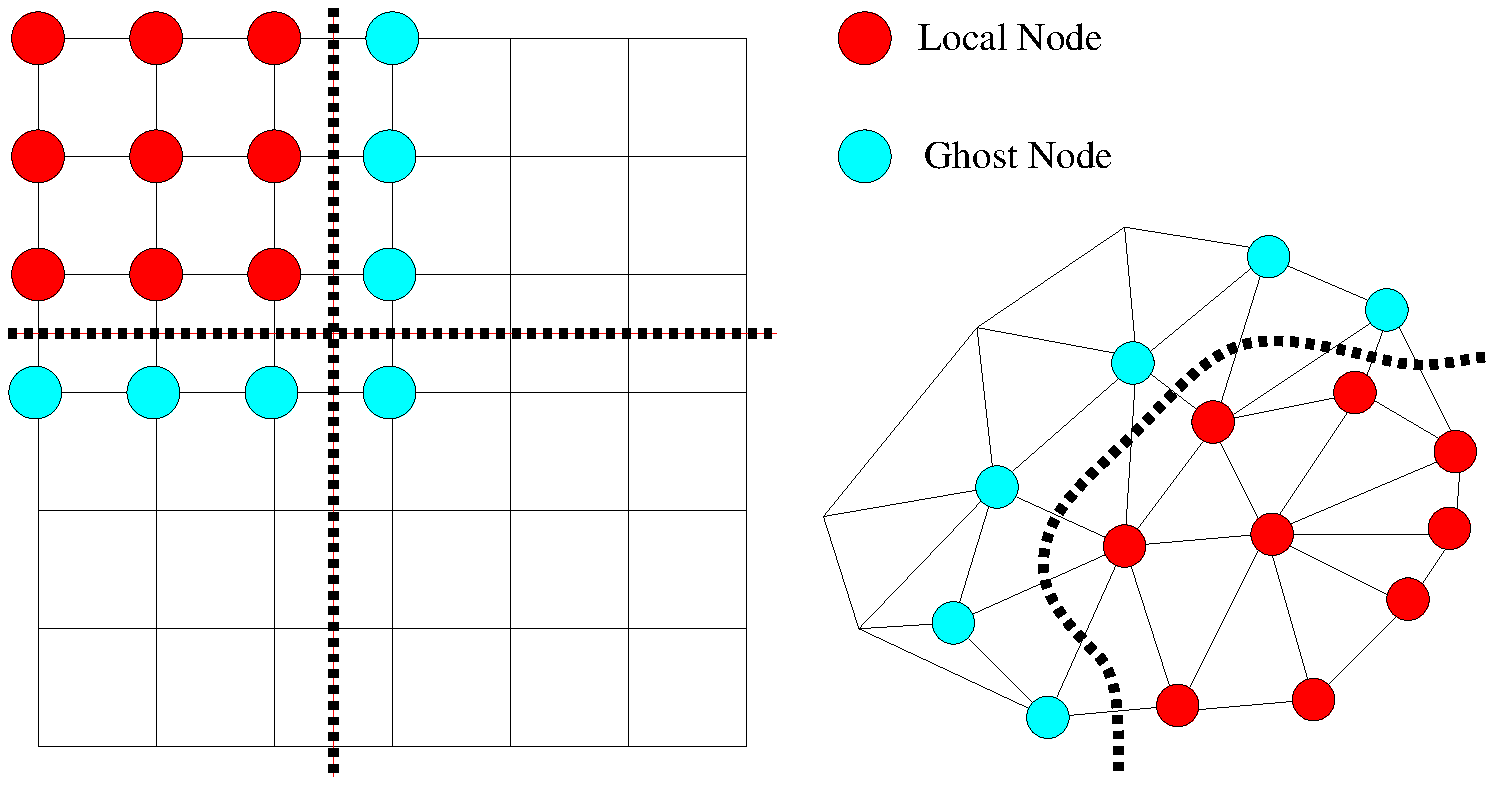
\includegraphics[width=4in]{figures/DA/GhostValues}
\end{center}
}

\begin{frame}{DA Global Numberings}

\begin{center}
\begin{tabular}{cc}
\begin{tabular}{c}
\begin{tabular}{|ccc|cc|}
\hline
\multicolumn{3}{|c|}{Proc 2} & \multicolumn{2}{c|}{Proc 3} \\
\hline
25 & 26 & 27 & 28 & 29 \\
20 & 21 & 22 & 23 & 24 \\
15 & 16 & 17 & 18 & 19 \\
\hline
10 & 11 & 12 & 13 & 14 \\
 5 &  6 &  7 &  8 &  9 \\
 0 &  1 &  2 &  3 &  4 \\
\hline
\multicolumn{3}{|c|}{Proc 0} & \multicolumn{2}{c|}{Proc 1} \\
\hline
\end{tabular} \\
Natural numbering
\end{tabular}
& 
\begin{tabular}{c}
\begin{tabular}{|ccc|cc|}
\hline
\multicolumn{3}{|c|}{Proc 2} & \multicolumn{2}{c|}{Proc 3} \\
\hline
21 & 22 & 23 & 28 & 29 \\
18 & 19 & 20 & 26 & 27 \\
15 & 16 & 17 & 24 & 25 \\
\hline
 6 &  7 &  8 & 13 & 14 \\
 3 &  4 &  5 & 11 & 12 \\
 0 &  1 &  2 &  9 & 10 \\
\hline
\multicolumn{3}{|c|}{Proc 0} & \multicolumn{2}{c|}{Proc 1} \\
\hline
\end{tabular}\\
PETSc numbering
\end{tabular}
\end{tabular}
\end{center}
\end{frame}

\begin{frame}{DMDA Global vs. Local Numbering}

\begin{itemize}
  \item {\bf Global}: Each vertex has a unique id belongs on a unique process

  \item {\bf Local}: Numbering includes vertices from neighboring processes
  \begin{itemize}
    \item These are called \cyan{ghost} vertices
  \end{itemize}
\end{itemize}

\begin{center}
\begin{tabular}{cc}
\begin{tabular}{c}
\begin{tabular}{|ccc|cc|}
\hline
\multicolumn{3}{|c|}{Proc 2} & \multicolumn{2}{c|}{Proc 3} \\
\hline
 X &  X &  X &  X &  X \\
 X &  X &  X &  X &  X \\
\cyan{12} & \cyan{13} & \cyan{14} & \cyan{15} &  X \\
\hline
 8 &  9 & 10 & \cyan{11} &  X \\
 4 &  5 &  6 &  \cyan{7} &  X \\
 0 &  1 &  2 &  \cyan{3} &  X \\
\hline
\multicolumn{3}{|c|}{Proc 0} & \multicolumn{2}{c|}{Proc 1} \\
\hline
\end{tabular} \\
Local numbering
\end{tabular}
& 
\begin{tabular}{c}
\begin{tabular}{|ccc|cc|}
\hline
\multicolumn{3}{|c|}{Proc 2} & \multicolumn{2}{c|}{Proc 3} \\
\hline
21 & 22 & 23 & 28 & 29 \\
18 & 19 & 20 & 26 & 27 \\
15 & 16 & 17 & 24 & 25 \\
\hline
 6 &  7 &  8 & 13 & 14 \\
 3 &  4 &  5 & 11 & 12 \\
 0 &  1 &  2 &  9 & 10 \\
\hline
\multicolumn{3}{|c|}{Proc 0} & \multicolumn{2}{c|}{Proc 1} \\
\hline
\end{tabular}\\
Global numbering
\end{tabular}
\end{tabular}
\end{center}
\end{frame}

\frame{
\frametitle{DM Vectors}

\begin{itemize}
  \item The DM object contains only layout (topology) information
  \begin{itemize}
    \item All field data is contained in PETSc {\kb Vec}s
  \end{itemize}

  \item Global vectors are parallel 
  \begin{itemize}
    \item Each process stores a unique local portion
    \item {\kb DMCreateGlobalVector(DM dm, Vec *gvec)}
  \end{itemize}

  \item Local vectors are sequential (and usually temporary)
  \begin{itemize}
    \item Each process stores its local portion plus ghost values
    \item {\kb DMCreateLocalVector(DM dm, Vec *lvec)}
    \item includes ghost values!
  \end{itemize}

  \item Coordinate vectors store the mesh geometry
    \begin{itemize}
    \item \code{DMDAGetCoordinates(DM dm, Vec *coords)}
    \item Can be manipulated with their own DMDA \\
      \code{DMDAGetCoordinateDA(DM dm,DM *cda)}
    \end{itemize}
\end{itemize}
}

\begin{frame}{Updating Ghosts}

Two-step process enables overlapping\\
computation and communication

\medskip

\begin{itemize}
  \item {\kb DMGlobalToLocalBegin(dm, gvec, mode, lvec)}
  \begin{itemize}
    \item {\kb gvec} provides the data 
    \item {\kb mode} is either {\kb INSERT\_VALUES} or {\kb ADD\_VALUES}
    \item {\kb lvec} holds the local and ghost values
  \end{itemize}

  \item {\kb DMGlobalToLocalEnd(dm, gvec, mode, lvec)}
  \begin{itemize}
    \item Finishes the communication
  \end{itemize}
\end{itemize}

\medskip

The process can be reversed with {\kb DMLocalToGlobalBegin()} and {\kb DMLocalToGlobalEnd()}.
\end{frame}

\frame{
\frametitle{DMDA Stencils}

Both the \blue{box} stencil and \blue{star} stencil are available.

\begin{center}
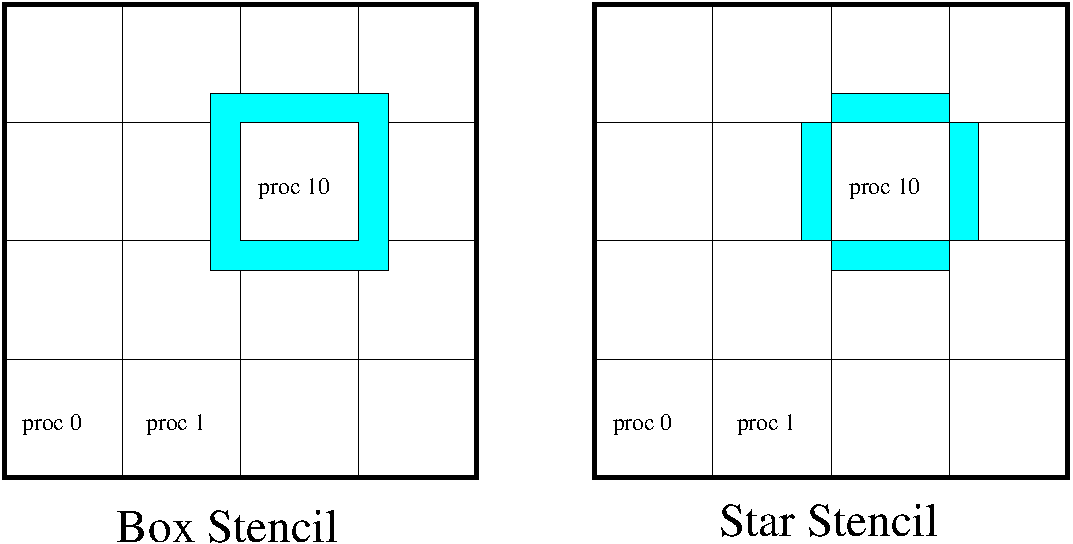
\includegraphics[width=4.5in]{figures/DA/Stencils}
\end{center}
}

\frame{
\frametitle{Creating a DMDA}

{\small \kb DMDACreate2d(comm, xbdy, ybdy, type, M, N, m, n, \\
\qquad\qquad\qquad  dof, s, lm[], ln[], DA *da)}
\begin{columns}\begin{column}{0.15\textwidth}\end{column}\begin{column}{0.85\textwidth}
  \begin{itemize}
  \item[{\kb xbdy,ybdy}:] Specifies periodicity or ghost cells
  \begin{itemize}
    \item {\kb DMDA\_BOUNDARY\_NONE}, {\kb DMDA\_BOUNDARY\_GHOSTED}, {\kb DMDA\_BOUNDARY\_MIRROR}, {\kb DMDA\_BOUNDARY\_PERIODIC}
  \end{itemize}
  \item[{\kb type}:] Specifies stencil
  \begin{itemize}
    \item {\kb DMDA\_STENCIL\_BOX} or {\kb DMDA\_STENCIL\_STAR}
  \end{itemize}
  \item[{\kb M,N}:] Number of grid points in x/y-direction
  \item[{\kb m,n}:] Number of processes in x/y-direction
  \item[{\kb dof}:] Degrees of freedom per node
  \item[{\kb s}:] The stencil width
  \item[{\kb lm,ln}:] Alternative array of local sizes
  \begin{itemize}
    \item Use {\kb PETSC\_NULL} for the default
  \end{itemize}
\end{itemize}
\end{column} \end{columns}
}

\begin{frame}{Working with the local form}
  Wouldn't it be nice if we could just write our code for the natural numbering?
  \begin{itemize}
  \item Yes, that's what \code{DMDAVecGetArray()} is for.
  \item Also, DMDA offers \emph{local} callback functions
    \begin{itemize}
    \item \code{FormFunctionLocal()}, set by \code{DMDASetLocalFunction()}
      
      \medskip
      
    \item \code{FormJacobianLocal()}, set by \code{DMDASetLocalJacobian()}
    \end{itemize}

    \bigskip

  \item When PETSc needs to evaluate the nonlinear residual $F(x)$,
    \begin{itemize}
    \item Each process evaluates the local residual

      \medskip

    \item PETSc assembles the global residual automatically
      \begin{itemize}
      \item Uses \code{DMLocalToGlobal()} method
      \end{itemize}
    \end{itemize}
  \end{itemize}
\end{frame}

\frame{
\frametitle{DA Local Function}

The user provided function which calculates the nonlinear residual in 2D has signature \\
{\kb PetscErrorCode (*lfunc)(DALocalInfo *info, \\
  \qquad \qquad \qquad Field **x, Field **r, void *ctx)}
\begin{columns}\begin{column}{0.15\textwidth}\end{column}\begin{column}{0.85\textwidth}
\begin{itemize}
  \item[{\kb info}:] All layout and numbering information
  \item[{\kb x}:] The current solution
  \begin{itemize}
    \item Notice that it is a multidimensional array
  \end{itemize}
  \item[ {\kb r}:] The residual
  \item[ {\kb ctx}:] The user context passed to {\kb DASetLocalFunction()}
\end{itemize}
\end{column}\end{columns}

\bigskip

The local DA function is activated by calling
\begin{center}
  {\kb SNESSetFunction(snes, r, SNESDAFormFunction, ctx)}
\end{center}
}

\begin{frame}[fragile]
\frametitle{Bratu Residual Evaluation}

\begin{equation*}
  -\Delta u - \lambda e^{u} = 0
\end{equation*}

\small
\begin{minted}[fontsize=\footnotesize]{c}
BratuResidualLocal(DMDALocalInfo *info,Field **x,Field **f,
                   UserCtx *user)
{
  /* Not Shown: Handle boundaries */
  /* Compute over the interior points */
  for(j = info->ys; j < info->ys+info->ym; j++) {
    for(i = info->xs; i < info->xs+info->xm; i++) {
      u       = x[j][i];
      u_xx    = (2.0*u - x[j][i-1] - x[j][i+1])*hydhx;
      u_yy    = (2.0*u - x[j-1][i] - x[j+1][i])*hxdhy;
      f[j][i] = u_xx + u_yy - hx*hy*lambda*exp(u);
    }
  }
}
\end{minted}

\begin{center}\small
\$PETSC\_DIR/src/snes/examples/tutorials/ex5.c
\end{center}
\end{frame}


\subsection{Profiling}
\begin{frame}{Profiling}

\begin{itemize}
  \item Use {\kb -log\_summary} for a performance profile
  \begin{itemize}
    \item Event timing
    \item Event flops
    \item Memory usage
    \item MPI messages
  \end{itemize}

  \item Call {\kb PetscLogStagePush()} and {\kb PetscLogStagePop()}
  \begin{itemize}
    \item User can add new stages
  \end{itemize}

  \item Call {\kb PetscLogEventBegin()} and {\kb PetscLogEventEnd()}
  \begin{itemize}
    \item User can add new events
  \end{itemize}

  \item Call {\kb PetscLogFlops()} to include your flops
\end{itemize}

\end{frame}

\begin{frame}[fragile]{Reading \code{-log\_summary}}
\begin{itemize}
\item
{\scriptsize
\begin{verbatim}
                         Max       Max/Min        Avg      Total 
Time (sec):           1.548e+02      1.00122   1.547e+02
Objects:              1.028e+03      1.00000   1.028e+03
Flops:                1.519e+10      1.01953   1.505e+10  1.204e+11
Flops/sec:            9.814e+07      1.01829   9.727e+07  7.782e+08
MPI Messages:         8.854e+03      1.00556   8.819e+03  7.055e+04
MPI Message Lengths:  1.936e+08      1.00950   2.185e+04  1.541e+09
MPI Reductions:       2.799e+03      1.00000
\end{verbatim}}
\item Also a summary per stage
\item Memory usage per stage (based on when it was allocated)
\item Time, messages, reductions, balance, flops per event per stage
\item Always send \code{-log\_summary} when asking \\
  performance questions on mailing list
\end{itemize}
\end{frame}

\begin{frame}[fragile]{Reading \code{-log\_summary}}
\begin{Verbatim}[formatcom=\tiny]
Event                Count      Time (sec)     Flops                             --- Global ---  --- Stage ---   Total
                   Max Ratio  Max     Ratio   Max  Ratio  Mess   Avg len Reduct  %T %F %M %L %R  %T %F %M %L %R Mflop/s
------------------------------------------------------------------------------------------------------------------------
--- Event Stage 1: Full solve
VecDot                43 1.0 4.8879e-02 8.3 1.77e+06 1.0 0.0e+00 0.0e+00 4.3e+01  0  0  0  0  0   0  0  0  0  1 73954
VecMDot             1747 1.0 1.3021e+00 4.6 8.16e+07 1.0 0.0e+00 0.0e+00 1.7e+03  0  1  0  0 14   1  1  0  0 27 128346
VecNorm             3972 1.0 1.5460e+00 2.5 8.48e+07 1.0 0.0e+00 0.0e+00 4.0e+03  0  1  0  0 31   1  1  0  0 61 112366
VecScale            3261 1.0 1.6703e-01 1.0 3.38e+07 1.0 0.0e+00 0.0e+00 0.0e+00  0  0  0  0  0   0  0  0  0  0 414021
VecScatterBegin     4503 1.0 4.0440e-01 1.0 0.00e+00 0.0 6.1e+07 2.0e+03 0.0e+00  0  0 50 26  0   0  0 96 53  0     0
VecScatterEnd       4503 1.0 2.8207e+00 6.4 0.00e+00 0.0 0.0e+00 0.0e+00 0.0e+00  0  0  0  0  0   0  0  0  0  0     0
MatMult             3001 1.0 3.2634e+01 1.1 3.68e+09 1.1 4.9e+07 2.3e+03 0.0e+00 11 22 40 24  0  22 44 78 49  0 220314
MatMultAdd           604 1.0 6.0195e-01 1.0 5.66e+07 1.0 3.7e+06 1.3e+02 0.0e+00  0  0  3  0  0   0  1  6  0  0 192658
MatMultTranspose     676 1.0 1.3220e+00 1.6 6.50e+07 1.0 4.2e+06 1.4e+02 0.0e+00  0  0  3  0  0   1  1  7  0  0 100638
MatSolve            3020 1.0 2.5957e+01 1.0 3.25e+09 1.0 0.0e+00 0.0e+00 0.0e+00  9 21  0  0  0  18 41  0  0  0 256792
MatCholFctrSym         3 1.0 2.8324e-04 1.0 0.00e+00 0.0 0.0e+00 0.0e+00 0.0e+00  0  0  0  0  0   0  0  0  0  0     0
MatCholFctrNum        69 1.0 5.7241e+00 1.0 6.75e+08 1.0 0.0e+00 0.0e+00 0.0e+00  2  4  0  0  0   4  9  0  0  0 241671
MatAssemblyBegin     119 1.0 2.8250e+00 1.5 0.00e+00 0.0 2.1e+06 5.4e+04 3.1e+02  1  0  2 24  2   2  0  3 47  5     0
MatAssemblyEnd       119 1.0 1.9689e+00 1.4 0.00e+00 0.0 2.8e+05 1.3e+03 6.8e+01  1  0  0  0  1   1  0  0  0  1     0
SNESSolve              4 1.0 1.4302e+02 1.0 8.11e+09 1.0 6.3e+07 3.8e+03 6.3e+03 51 50 52 50 50  99100 99100 97 113626
SNESLineSearch        43 1.0 1.5116e+01 1.0 1.05e+08 1.1 2.4e+06 3.6e+03 1.8e+02  5  1  2  2  1  10  1  4  4  3 13592
SNESFunctionEval      55 1.0 1.4930e+01 1.0 0.00e+00 0.0 1.8e+06 3.3e+03 8.0e+00  5  0  1  1  0  10  0  3  3  0     0
SNESJacobianEval      43 1.0 3.7077e+01 1.0 7.77e+06 1.0 4.3e+06 2.6e+04 3.0e+02 13  0  4 24  2  26  0  7 48  5   429
KSPGMRESOrthog      1747 1.0 1.5737e+00 2.9 1.63e+08 1.0 0.0e+00 0.0e+00 1.7e+03  1  1  0  0 14   1  2  0  0 27 212399
KSPSetup             224 1.0 2.1040e-02 1.0 0.00e+00 0.0 0.0e+00 0.0e+00 3.0e+01  0  0  0  0  0   0  0  0  0  0     0
KSPSolve              43 1.0 8.9988e+01 1.0 7.99e+09 1.0 5.6e+07 2.0e+03 5.8e+03 32 49 46 24 46  62 99 88 48 88 178078
PCSetUp              112 1.0 1.7354e+01 1.0 6.75e+08 1.0 0.0e+00 0.0e+00 8.7e+01  6  4  0  0  1  12  9  0  0  1 79715
PCSetUpOnBlocks     1208 1.0 5.8182e+00 1.0 6.75e+08 1.0 0.0e+00 0.0e+00 8.7e+01  2  4  0  0  1   4  9  0  0  1 237761
PCApply              276 1.0 7.1497e+01 1.0 7.14e+09 1.0 5.2e+07 1.8e+03 5.1e+03 25 44 42 20 41  49 88 81 39 79 200691
\end{Verbatim}
\end{frame}

\begin{frame}{Communication Costs}
  \begin{itemize}
  \item Reductions: usually part of Krylov method, latency limited
    \begin{itemize}
    \item \code{VecDot}
    \item \code{VecMDot}
    \item \code{VecNorm}
    \item \code{MatAssemblyBegin}
    \item Change algorithm (e.g. IBCGS)
    \end{itemize}
  \item Point-to-point (nearest neighbor), latency or bandwidth
    \begin{itemize}
    \item \code{VecScatter}
    \item \code{MatMult}
    \item \code{PCApply}
    \item \code{MatAssembly}
    \item \code{SNESFunctionEval}
    \item \code{SNESJacobianEval}
    \item Compute subdomain boundary fluxes redundantly
    \item Ghost exchange for all fields at once
    \item Better partition
    \end{itemize}
  \end{itemize}
\end{frame}


\subsection{Matrix Redux}
\begin{frame}{Matrices, redux}
What are PETSc matrices?
\begin{itemize}
\item Linear operators on finite dimensional vector spaces. (snarky)
  \item<2> Fundamental objects for storing stiffness matrices and Jacobians
  \item<2> Each process locally owns a contiguous set of rows
  \item<2> Supports many data types
  \begin{itemize}
    \item AIJ, Block AIJ, Symmetric AIJ, Block Diagonal, etc.
  \end{itemize}
  \item<2> Supports structures for many packages
  \begin{itemize}
    \item MUMPS, Spooles, SuperLU, UMFPack, DSCPack
  \end{itemize}
\end{itemize}
\end{frame}

\begin{frame}{How do I create matrices?}

\begin{itemize}
  \item {\kb MatCreate(MPI\_Comm, Mat *)}
  \item {\kb MatSetSizes(Mat, int m, int n, int M, int N)}
  \item {\kb MatSetType(Mat, MatType typeName)}
  \item {\kb MatSetFromOptions(Mat)}
  \begin{itemize}
    \item Can set the type at runtime
  \end{itemize}
  \item {\kb MatMPIBAIJSetPreallocation(Mat,...)} %(Mat,int bs,int d_nz,const int
                                %d_nnz[],int o_nz,const int o_nnz[])}
    \oneitem{important for assembly performance, more tomorrow}
  \item {\kb MatSetBlockSize(Mat, int bs)}
    \oneitem{for vector problems}
  \item {\kb MatSetValues(Mat,...)}
  \begin{itemize}
    \item {\bf MUST} be used, but does automatic communication
  \end{itemize}
\end{itemize}

\end{frame}

\begin{frame}{Matrix Polymorphism}

The PETSc {\kb Mat} has a single user interface,
\begin{itemize}
  \item Matrix assembly
  \begin{itemize}
    \item {\kb MatSetValues()}
  \end{itemize}

  \item Matrix-vector multiplication
  \begin{itemize}
    \item {\kb MatMult()}
  \end{itemize}

  \item Matrix viewing
  \begin{itemize}
    \item {\kb MatView()}
  \end{itemize}
\end{itemize}
but multiple underlying implementations.
\begin{itemize}
  \item AIJ, Block AIJ, Symmetric Block AIJ,
  \item Dense
  \item Matrix-Free
  \item etc.
\end{itemize}
A matrix is defined by its {\red{interface}}, not by its {\blue{data structure}}.

\end{frame}

\begin{frame}{Matrix Assembly}

\begin{itemize}
  \item A three step process
  \begin{itemize}
    \item Each process sets or adds values
    \item Begin communication to send values to the correct process
    \item Complete the communication
  \end{itemize}
  \item {\kb MatSetValues(Mat A, m, rows[], n, cols[], values[], mode)}
  \begin{itemize}
    \item {\kb mode} is either INSERT\_VALUES or ADD\_VALUES
    \item Logically dense block of values
  \end{itemize}
% TODO picture of MatSetValues
  \item Two phase assembly allows overlap of communication and computation
  \begin{itemize}
    \item {\kb MatAssemblyBegin(Mat m, type)}
    \item {\kb MatAssemblyEnd(Mat m, type)}
    \item {\kb type} is either MAT\_FLUSH\_ASSEMBLY or MAT\_FINAL\_ASSEMBLY
  \end{itemize}
  \item<2-> For vector problems\\
    {\kb MatSetValuesBlocked(Mat A, m, rows[], \\
      \qquad\qquad n, cols[], values[], mode)}
  \item<2-> The same assembly code can build matrices of different format
    \begin{itemize}
    \item choose format at run-time.
    \end{itemize}
\end{itemize}

\end{frame}

\begin{frame}[fragile]{One Way to Set the Elements of a Matrix}{Simple 3-point stencil for 1D Laplacian}
\small
\begin{minted}{c}
v[0] = -1.0; v[1] = 2.0; v[2] = -1.0;
if (rank == 0) {
  for(row = 0;  row < N; row++) {
    cols[0] = row-1; cols[1] = row; cols[2] = row+1;
    if (row == 0) {
      MatSetValues(A,1,&row,2,&cols[1],&v[1],INSERT_VALUES);
    } else if (row == N-1) {
      MatSetValues(A,1,&row,2,cols,v,INSERT_VALUES);
    } else {
      MatSetValues(A,1,&row,3,cols,v,INSERT_VALUES);
    }
  }
}
MatAssemblyBegin(A,MAT_FINAL_ASSEMBLY);
MatAssemblyEnd(A,MAT_FINAL_ASSEMBLY);
\end{minted}
\end{frame}

\begin{frame}[fragile]{A Better Way to Set the Elements of a Matrix}{Simple 3-point stencil for 1D Laplacian}
\small
\begin{minted}{c}
v[0] = -1.0; v[1] = 2.0; v[2] = -1.0;
for(row = start;  row < end; row++) {
  cols[0] = row-1; cols[1] = row; cols[2] = row+1;
  if (row == 0) {
    MatSetValues(A,1,&row,2,&cols[1],&v[1],INSERT_VALUES);
  } else if (row == N-1) {
    MatSetValues(A,1,&row,2,cols,v,INSERT_VALUES);
  } else {
    MatSetValues(A,1,&row,3,cols,v,INSERT_VALUES);
  }
}
MatAssemblyBegin(A, MAT_FINAL_ASSEMBLY);
MatAssemblyEnd(A, MAT_FINAL_ASSEMBLY);
\end{minted}
\end{frame}

\begin{frame}{Why Are PETSc Matrices That Way?}

\begin{itemize}
  \item No one data structure is appropriate for all problems
  \begin{itemize}
    \item Blocked and diagonal formats provide significant performance benefits
    \item PETSc has many formats and makes it easy to add new data structures
  \end{itemize}

  \item Assembly is difficult enough without worrying about partitioning
  \begin{itemize}
    \item PETSc provides parallel assembly routines
    \item Achieving high performance still requires making most operations local
    \item However, programs can be incrementally developed.
    \item {\kb MatPartitioning} and {\kb MatOrdering} can help
  \end{itemize}

  \item Matrix decomposition in contiguous chunks is simple
  \begin{itemize}
    \item Makes interoperation with other codes easier
    \item For other ordering, PETSc provides ``Application Orderings'' (AO)
  \end{itemize}
\end{itemize}

\end{frame}


\section*{Preliminary Conclusions}
\begin{frame}{Preliminary Conclusions}
  \begin{block}{PETSc can help you}
    \begin{itemize}
    \item solve algebraic and DAE problems in your application area
    \item rapidly develop efficient parallel code, can start from examples
    \item develop new solution methods and data structures
    \item debug and analyze performance
    \item advice on software design, solution algorithms, and performance
      \begin{itemize}
        \item Public questions: \url{petsc-users@mcs.anl.gov}, archived
        \item Private questions: \url{petsc-maint@mcs.anl.gov}, not archived
      \end{itemize}
    \end{itemize}
  \end{block}
  \begin{block}{You can help PETSc}
    \begin{itemize}
    \item report bugs and inconsistencies, or if you think there is a better way
    \item tell us if the documentation is inconsistent or unclear
    \item consider developing new algebraic methods as plugins, contribute if your idea works
    \end{itemize}
  \end{block}
\end{frame}


\part{Integration and Efficiency}
\section{Application Integration}
\begin{frame}{Application Integration}

\begin{itemize}
  \item Be willing to experiment with algorithms
  \begin{itemize}
    \item No optimality without interplay between physics and algorithmics
  \end{itemize}

  \item Adopt flexible, extensible programming
  \begin{itemize}
    \item Algorithms and data structures not hardwired
  \end{itemize}

  \item Be willing to play with the real code
  \begin{itemize}
    \item Toy models are rarely helpful
  \end{itemize}

  \item If possible, profile before integration
  \begin{itemize}
    \item Automatic in PETSc
  \end{itemize}
\end{itemize}

\end{frame}

\begin{frame}{Incorporating PETSc into existing codes}
  \begin{itemize}
  \item PETSc does not seize \code{main()}, does not control output
  \item Propogates errors from underlying packages, flexible error handling
  \item Nothing special about \code{MPI\_COMM\_WORLD}
  \item Can wrap existing data structures/algorithms
    \begin{itemize}
    \item \code{MatShell}, \code{PCShell}, full implementations
    \item \code{VecCreateMPIWithArray()}
    \item \code{MatCreateSeqAIJWithArrays()}
    \item Use an existing semi-implicit solver as a preconditioner
    \item Usually worthwhile to use native PETSc data structures \\
      unless you have a good reason not to
    \end{itemize}
  \item Uniform interfaces across languages
    \begin{itemize}
    \item C, C++, Fortran 77/90, Python, MATLAB
    \end{itemize}
  \item Do not have to use high level interfaces (\eg SNES, TS, DM)
    \begin{itemize}
    \item but PETSc can offer more if you do, like MFFD and SNES Test
    \end{itemize}
  \end{itemize}
\end{frame}

\begin{frame}{Integration Stages}

\begin{itemize}
  % I like the simile of VC as a will. It cheap, easy, someone will help you,
  % and if you die you are an idiot for not using one
  \item \red{Version Control}
  \begin{itemize}
    \item It is impossible to overemphasize
  \end{itemize}

  \item Initialization
  \begin{itemize}
    \item Linking to PETSc
  \end{itemize}

  \item Profiling
  \begin{itemize}
    \item Profile \red{before} changing
    \item Also incorporate command line processing
  \end{itemize}

  \item Linear Algebra
  \begin{itemize}
    \item First PETSc data structures
  \end{itemize}

  \item Solvers
  \begin{itemize}
    \item Very easy after linear algebra is integrated
  \end{itemize}
\end{itemize}

\end{frame}

\begin{frame}{Initialization}

\begin{itemize}
  \item Call {\kb PetscInitialize()}
  \begin{itemize}
    \item Setup static data and services
    \item Setup MPI if it is not already
    \item Can set \code{PETSC\_COMM\_WORLD} to use your communicator \\
      (can always use subcommunicators for each object)
  \end{itemize}

  \item Call {\kb PetscFinalize()}
  \begin{itemize}
    \item Calculates logging summary
    \item Can check for leaks/unused options
    \item Shutdown and release resources
  \end{itemize}

  \item Can only initialize PETSc once
\end{itemize}

\end{frame}

\begin{frame}{Matrix Memory Preallocation}
\begin{itemize}
  \item PETSc sparse matrices are dynamic data structures
  \begin{itemize}
    \item can add additional nonzeros freely
  \end{itemize}

  \item Dynamically adding many nonzeros 
  \begin{itemize}
    \item requires additional memory allocations
    \item requires copies
    \item can kill performance
  \end{itemize}

  \item Memory preallocation provides
  \begin{itemize}
    \item the freedom of dynamic data structures
    \item good performance
  \end{itemize}

  \item Easiest solution is to replicate the assembly code
  \begin{itemize}
    \item Remove computation, but preserve the indexing code
    \item Store set of columns for each row
  \end{itemize}

  \item Call preallocation routines for all datatypes
  \begin{itemize}
    \item {\kb MatSeqAIJSetPreallocation()}
    \item {\kb MatMPIBAIJSetPreallocation()}
    \item Only the relevant data will be used
  \end{itemize}
\end{itemize}
\end{frame}

\begin{frame}{Sequential Sparse Matrices}
{\kb MatSeqAIJSetPreallocation(Mat A, int nz, int nnz[])}
\hbox{\qquad
\vbox{
\begin{itemize}
  \item[nz:] expected number of nonzeros in any row
  \item[nnz(i):] expected number of nonzeros in row i
\end{itemize}
}
}

\begin{center}
%\includegraphics[width=2in]{figures/Mat/serialSparseMatrix_bcsstk32}
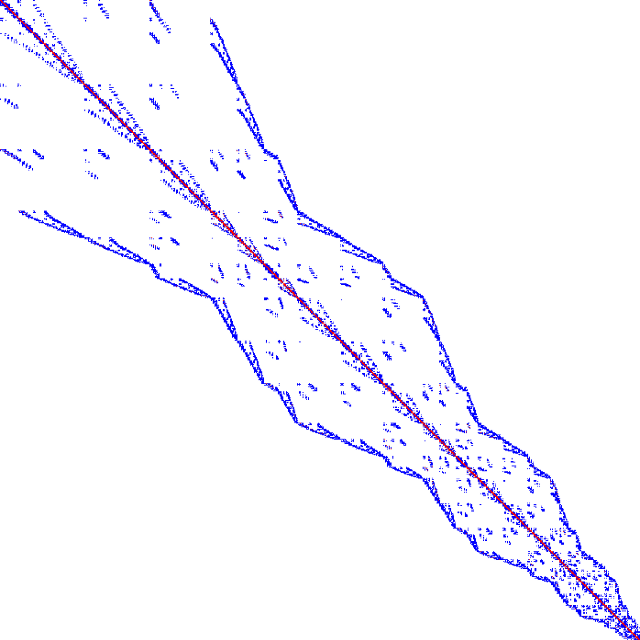
\includegraphics[width=.5\textwidth]{figures/EllipRCMSquare}
\end{center}
\end{frame}

\begin{frame}{Parallel Sparse Matrix}
\begin{itemize}
  \item Each process locally owns a submatrix of contiguous global rows
  \item Each submatrix consists of diagonal and off-diagonal parts
\end{itemize}

\begin{center}
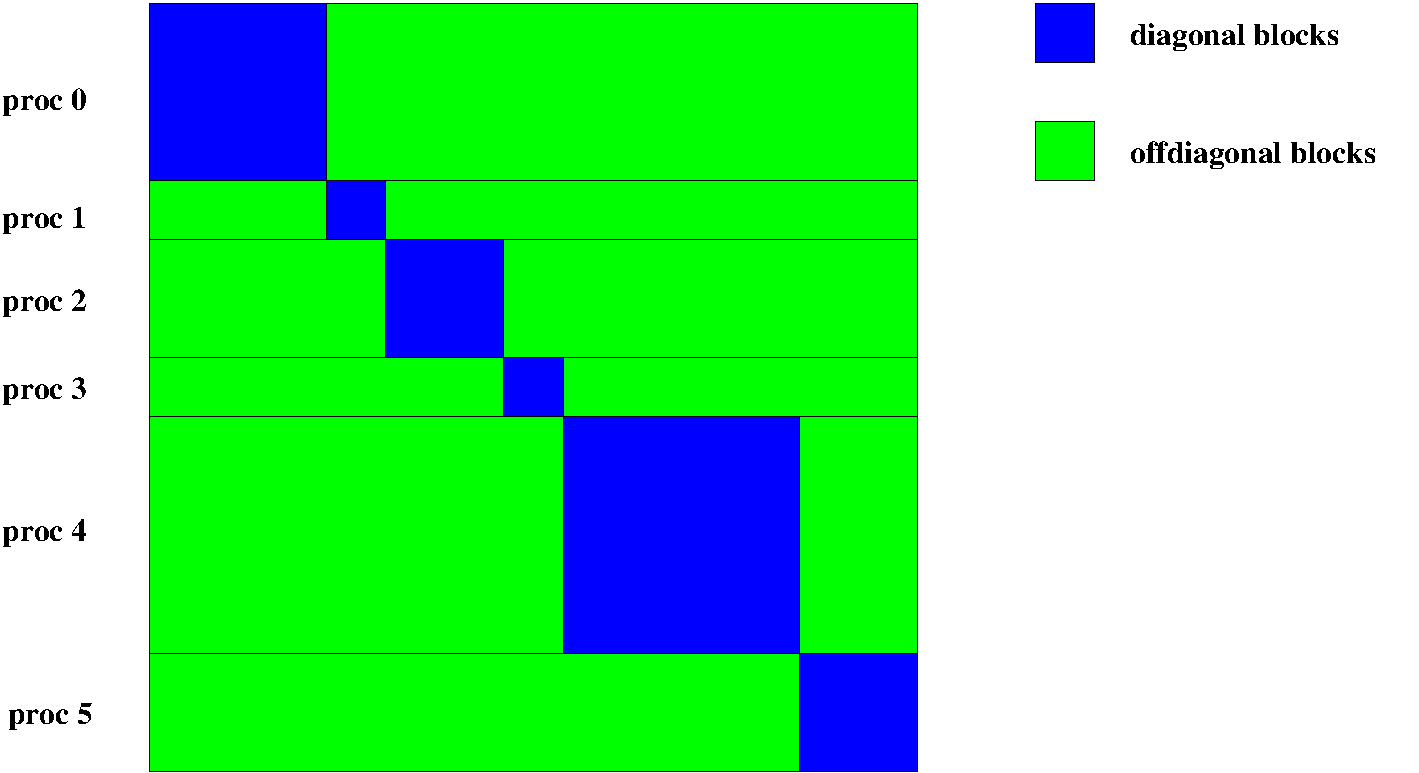
\includegraphics[width=3.5in]{figures/Mat/parallelSparseMatrix}
\end{center}

\begin{itemize}
  \item {\kb MatGetOwnershipRange(Mat A,int *start,int *end)}
  \begin{itemize}
    \item[{\kb start}:] first locally owned row of global matrix
    \item[{\kb end-1}:] last locally owned row of global matrix
  \end{itemize}
\end{itemize}
\end{frame}

\begin{frame}{Parallel Sparse Matrices}
\hbox{
\quad
\vbox{
{\kb MatMPIAIJSetPreallocation(Mat A, int dnz, int dnnz[], \\
  \qquad \qquad int onz, int onnz[])}
\begin{itemize}
  \item[dnz:] expected number of nonzeros in any row in the diagonal block
  \item[dnnz(i):] expected number of nonzeros in row i in the diagonal block
  \item[onz:] expected number of nonzeros in any row in the offdiagonal portion
  \item[onnz(i):] expected number of nonzeros in row i in the offdiagonal portion
\end{itemize}
}
}
\end{frame}

\begin{frame}{Verifying Preallocation}
\begin{itemize}
  \item Use runtime options \\
    {\kb -mat\_new\_nonzero\_location\_err} \\
    {\kb -mat\_new\_nonzero\_allocation\_err}
  \item Use runtime option {\kb -info}
  \item Output: \\
{\kb
  $[$proc \#$]$ Matrix size: \%d X \%d; storage space: \%d unneeded, \%d used \\
  $[$proc \#$]$ Number of mallocs during MatSetValues( )  is \%d
}
\end{itemize}

\bigskip

\begin{center}
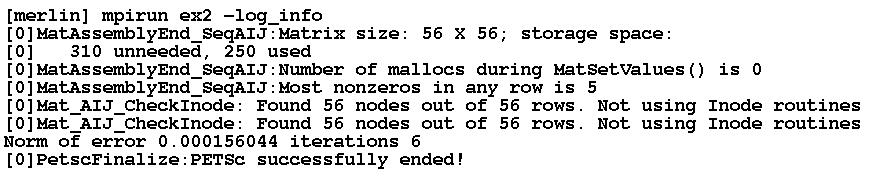
\includegraphics[width=5in]{figures/PETSc/logInfoOutput}
\end{center}
\end{frame}

\begin{frame}{Block and symmetric formats}
  \begin{itemize}
  \item BAIJ
    \begin{itemize}
    \item Like AIJ, but uses static block size
    \item Preallocation is like AIJ, but just one index per block
    \end{itemize}
  \item SBAIJ
    \begin{itemize}
    \item Only stores upper triangular part
    \item Preallocation needs number of nonzeros in upper triangular \\
      parts of on- and off-diagonal blocks
    \end{itemize}
  \item \code{MatSetValuesBlocked()}
    \begin{itemize}
    \item Better performance with blocked formats
    \item Also works with scalar formats, if \code{MatSetBlockSize()} was called
    \item Variants \code{MatSetValuesBlockedLocal()}, \code{MatSetValuesBlockedStencil()}
    \item Change matrix format at runtime, don't need to touch assembly code
    \end{itemize}
  \end{itemize}
\end{frame}

\begin{frame}{Linear Solvers}{Krylov Methods}

\begin{itemize}
  \item Using PETSc linear algebra, just add:
  \begin{itemize}
    \item {\kb KSPSetOperators(KSP ksp, Mat A, Mat M, MatStructure flag)}
    \item {\kb KSPSolve(KSP ksp, Vec b, Vec x)}
  \end{itemize}

  \item Can access subobjects
  \begin{itemize}
    \item {\kb KSPGetPC(KSP ksp, PC *pc)}
  \end{itemize}

  \item Preconditioners must obey PETSc interface
  \begin{itemize}
    \item Basically just the KSP interface
  \end{itemize}

  \item Can change solver dynamically from the command line, {\kb -ksp\_type}
\end{itemize}

\end{frame}

\begin{frame}{Nonlinear Solvers}{Newton and Picard Methods}

\begin{itemize}
  \item Using PETSc linear algebra, just add:
  \begin{itemize}
    \item {\kb SNESSetFunction(SNES snes, Vec r, residualFunc, void *ctx)}
    \item {\kb SNESSetJacobian(SNES snes, Mat A, Mat M, jacFunc, void *ctx)}
    \item {\kb SNESSolve(SNES snes, Vec b, Vec x)}
  \end{itemize}

  \item Can access subobjects
  \begin{itemize}
    \item {\kb SNESGetKSP(SNES snes, KSP *ksp)}
  \end{itemize}

  \item Can customize subobjects from the cmd line
  \begin{itemize}
    \item Set the subdomain preconditioner to ILU with {\kb -sub\_pc\_type ilu} 
  \end{itemize}
\end{itemize}

\end{frame}


\section{Performance and Scalability}
\begin{frame}{Bottlenecks of (Jacobian-free) Newton-Krylov}
  \begin{columns}
    \begin{column}{0.4\textwidth}
      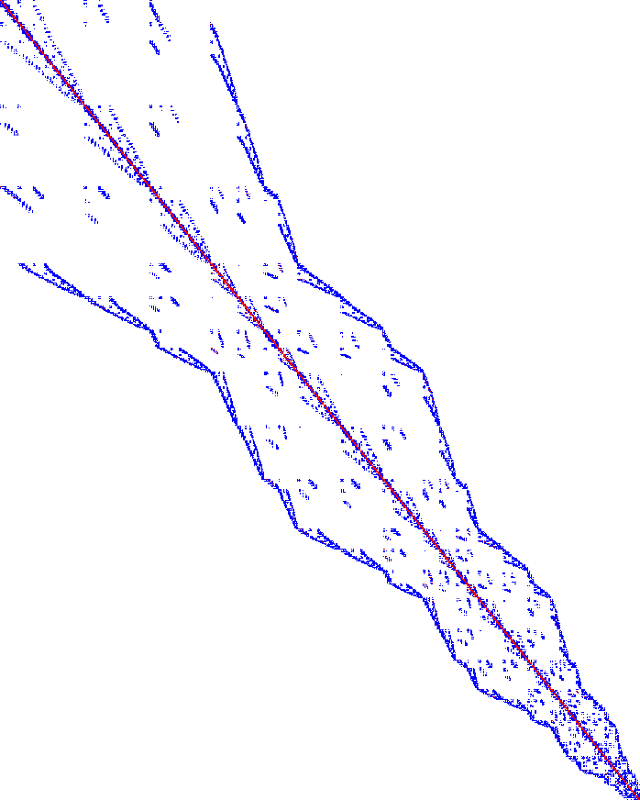
\includegraphics[width=1.15\textwidth]{figures/Dohp/EllipRCM}
    \end{column}
    \begin{column}{0.6\textwidth}
      \begin{itemize}
      \item Matrix assembly
        \begin{itemize}
        \item integration/fluxes: FPU
        \item insertion: memory/branching
        \end{itemize}
      \item Preconditioner setup
        \begin{itemize}
        \item coarse level operators
        \item overlapping subdomains
        \item (incomplete) factorization
        \end{itemize}
      \item Preconditioner application
        \begin{itemize}
        \item triangular solves/relaxation: memory
        \item coarse levels: network latency
        \end{itemize}
      \item Matrix multiplication
        \begin{itemize}
        \item Sparse storage: memory
        \item Matrix-free: FPU
        \end{itemize}
      \item Globalization
      \end{itemize}
    \end{column}
  \end{columns}
\end{frame}

\begin{frame}{Scalability definitions}
  \begin{columns}
    \begin{column}{0.5\textwidth}
      {\large Strong scalability}
      \begin{itemize}
      \item Fixed problem size
      \item execution time $T$ inversely proportional to number of processors $p$
      \end{itemize}
    \end{column}
    \begin{column}{0.5\textwidth}
      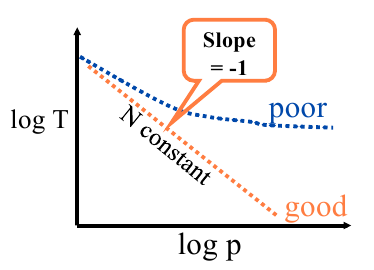
\includegraphics[width=\textwidth]{figures/KeyesStrongScaling.png}
    \end{column}
  \end{columns}
  \begin{columns}
    \begin{column}{0.5\textwidth}
      {\large Weak scalability}
      \begin{itemize}
      \item Fixed problem size per processor
      \item execution time constant as problem size increases
      \end{itemize}
    \end{column}
    \begin{column}{0.5\textwidth}
      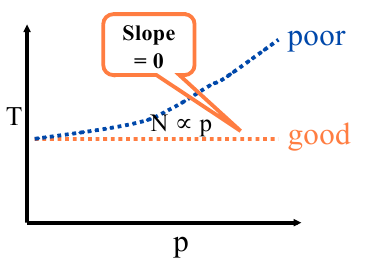
\includegraphics[width=\textwidth]{figures/KeyesWeakScaling.png}
    \end{column}
  \end{columns}
\end{frame}

\begin{frame}{Scalability Warning}
  \begin{quote}\Large \centering
    The easiest way to make software scalable \\
    is to make it sequentially inefficient. \\
    (Gropp 1999)
  \end{quote}

  \begin{itemize}
  \item We really want \alert{efficient} software
  \item Need a performance model
    \begin{itemize}
    \item memory bandwidth and latency
    \item algorithmically critical operations (\eg dot products, scatters)
    \item floating point unit
    \end{itemize}
  \item Scalability shows marginal benefit of adding more cores, nothing more
  \item Constants hidden in the choice of algorithm
  \item Constants hidden in implementation
  \end{itemize}
\end{frame}

\subsection{Memory hierarchy}
\begin{frame} %{CPU Architecture}
  \begin{columns}
    \begin{column}{0.5\textwidth}
      {\centering Intel Clowertown \\
      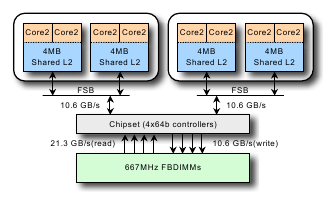
\includegraphics[width=\textwidth]{figures/hardware/IntelClovertown} }
    \begin{itemize}
    \item 75 Gflop/s
    \item 21 GB/s bandwidth
    \item thread + instruction level parallelism
    \item vector instructions (SSE)
    \end{itemize}
    \end{column}
    \begin{column}{0.5\textwidth}
      {\centering       AMD Opteron \\
      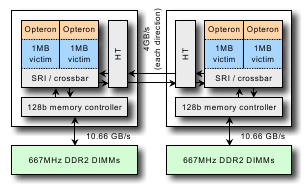
\includegraphics[width=\textwidth]{figures/hardware/AMDOpteron} }
    \begin{itemize}
    \item 17 Gflop/s
    \item 21 GB/s bandwidth
    \item thread + instruction level parallelism
    \item vector instructions (SSE)
    \end{itemize}
    \end{column}
  \end{columns}
\end{frame}

\begin{frame}{Hardware capabilities}
  \begin{columns}
    \begin{column}{0.5\textwidth}
      \begin{block}{Floating point unit}
        Recent Intel: each core can issue
        \begin{itemize}
        \item 1 packed add (latency 3)
        \item 1 packed mult (latency 5)
        \item One can include an aligned read
        \item Out of Order execution
        \item Peak: 10 Gflop/s (\texttt{double})
        \end{itemize}
      \end{block}
    \end{column}
    \begin{column}{0.5\textwidth}
      \begin{block}{Memory}
        \begin{itemize}
        \item $\sim 250$ cycle latency
        \item 5.3 GB/s bandwidth
        \item 1 \texttt{double} load / 3.7 cycles
        \item Pay by the cache line (32/64 B)
        \item L2 cache: $\sim 10$ cycle latency
        \end{itemize}
      \end{block}
    \end{column}
  \end{columns}
  \begin{block}{}%<2>{\alert{\Large It's \textbf{all} about the memory hierarchy}}
    \centering
    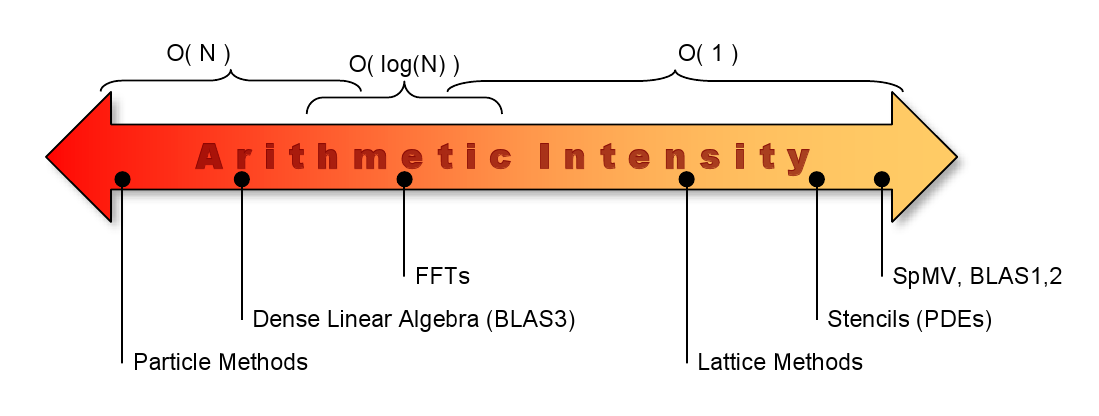
\includegraphics[width=0.85\textwidth]{figures/OlikerArithmeticIntensity} \\
    \vspace{-1em}
    {\tiny (Oliker et al. 2008)}
  \end{block}
\end{frame}

\frame{
  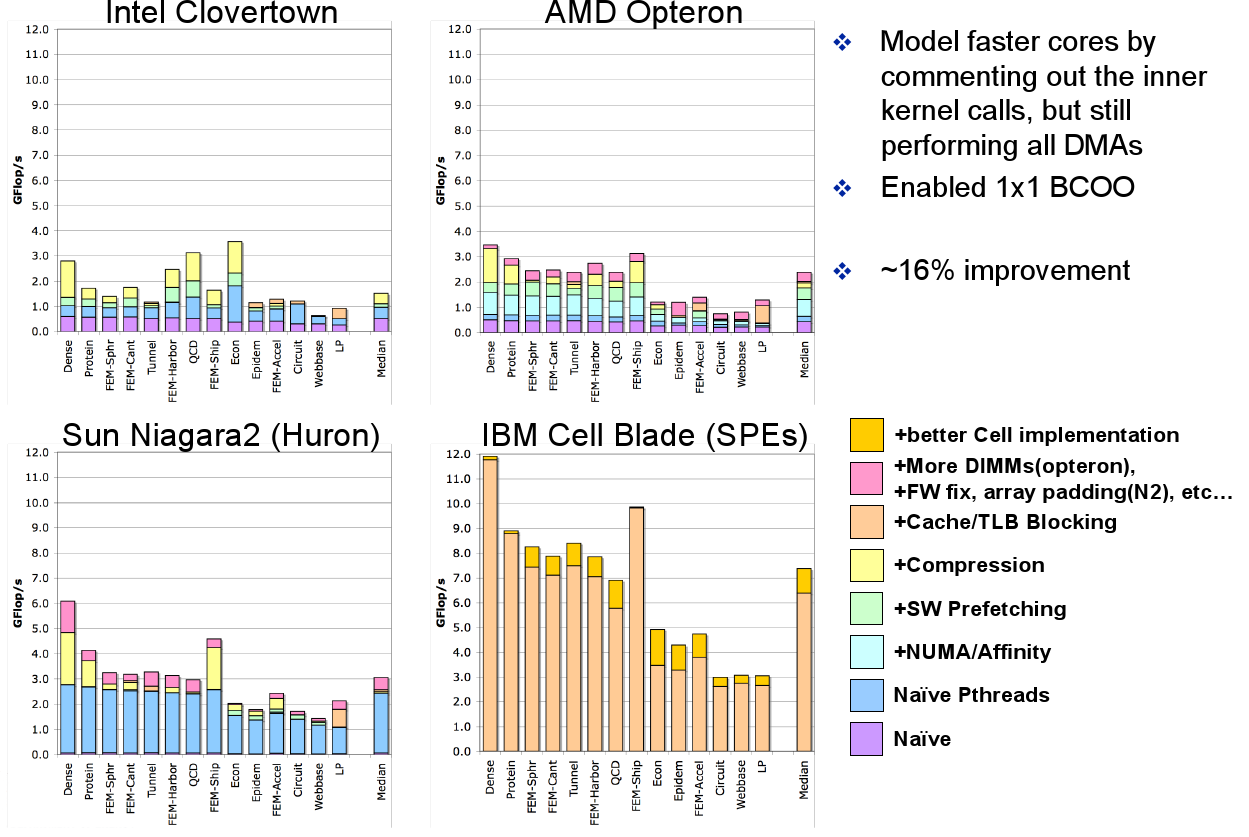
\includegraphics[width=\textwidth]{figures/OlikerSpMv} \\
  {\tiny (Oliker et al. \emph{Multi-core Optimization of Sparse Matrix Vector Multiplication}, 2008)}
}

\begin{frame}[fragile]{Sparse Mat-Vec performance model}
  \begin{block}{Compressed Sparse Row format (AIJ)}
    For $m \times n$ matrix with $N$ nonzeros
    \begin{itemize}
    \item[ai] row starts, length $m+1$
    \item[aj] column indices, length $N$, range $[0,n-1)$
    \item[aa] nonzero entries, length $N$, scalar values
    \end{itemize}
  \end{block}
\begin{columns}
\begin{column}{0.3\textwidth}
\[y \gets y + A x\]
\end{column}
\begin{column}{0.7\textwidth}
\begin{lstlisting}
  for (i=0; i<m; i++)
    for (j=ai[i]; j<ai[i+1]; j++)
      y[i] += aa[j] * x[aj[j]];
    \end{lstlisting}
  \end{column}
\end{columns}
  \begin{itemize}
  \item One add and one multiply per inner loop
  \item Scalar \code{aa[j]} and integer \code{aj[j]} only used once
  \item Must load \code{aj[j]} to read from \code{x}, may not reuse cache well
  \end{itemize}
\end{frame}

\begin{frame}[shrink=1]{Memory Bandwidth}
\begin{itemize}
\item Stream Triad benchmark (GB/s): $\bm w \gets \alpha \bm x + \bm y$
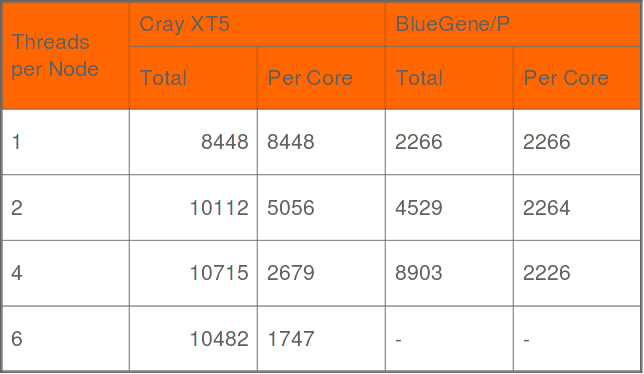
\includegraphics[width=0.8\textwidth]{figures/StreamTriadXT5VsBGP} \\
\item Sparse matrix-vector product: 6 bytes per flop
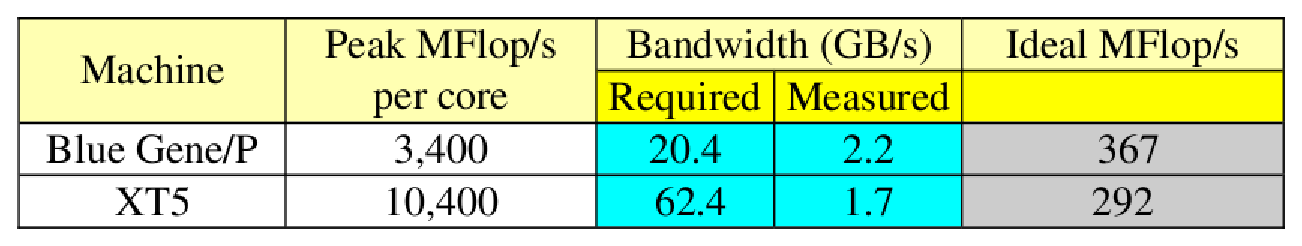
\includegraphics[width=0.8\textwidth]{figures/SparseMatVec} \\
%{\footnotesize (from Dinesh Kaushik)}
\end{itemize}
\end{frame}



\begin{frame}{Optimizing Sparse Mat-Vec}
  \begin{itemize}
  \item Order unknows so that vector reuses cache (Reverse Cuthill-McKee)
    \begin{itemize}
    \item Optimal: $\frac{(2 \text{ flops})(\text{bandwidth})}{\texttt{sizeof(Scalar)} + \texttt{sizeof(Int)}}$
    \item Usually improves strength of ILU and SOR
    \end{itemize}
  \item Coalesce indices for adjacent rows with same nonzero pattern (Inodes)
    \begin{itemize}
    \item Optimal: $\frac{(2 \text{ flops})(\text{bandwidth})}{\texttt{sizeof(Scalar)} + \texttt{sizeof(Int)}/i}$
    \item Can do block SOR (much stronger than scalar SOR)
    \item Default in PETSc, turn off with \code{-mat\_no\_inode}
    \item Requires ordering unknowns so that fields are interlaced, this
      is (much) better for memory use anyway
    \end{itemize}
  \item Use explicit blocking, hold one index per block (BAIJ format)
    \begin{itemize}
    \item Optimal: $\frac{(2 \text{ flops})(\text{bandwidth})}{\texttt{sizeof(Scalar)} + \texttt{sizeof(Int)}/b^2}$
    \item Block SOR and factorization
    \item Symbolic factorization works with blocks (much cheaper)
    \item Very regular memory access, unrolled dense kernels
    \item Faster insertion: \code{MatSetValuesBlocked()}
    \end{itemize}
  \end{itemize}
\end{frame}

\begin{frame}[shrink=5]{Performance of assembled versus unassembled}
  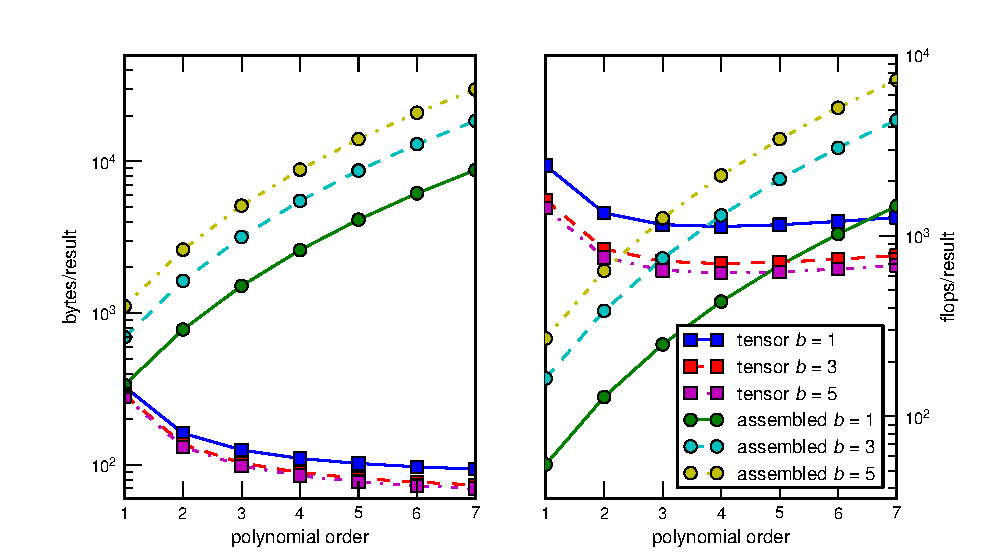
\includegraphics[width=\textwidth]{figures/TensorVsAssembly} \\
  \begin{itemize}
  \item Arithmetic intensity for $\Qk p$ elements
    \begin{itemize}
    \item $\le \frac 1 4$ (assembled), $\approx 10$ (unassembled), $\approx 4$ (hardware)
    \end{itemize}
  \item store Jacobian information at Quass quadrature points, can use AD
  \end{itemize}
\end{frame}

\begin{frame}{Optimizing unassembled Mat-Vec}
  \begin{itemize}
  \item High order spatial discretizations do more work per node
    \begin{itemize}
    \item Dense tensor product kernel (like small BLAS3)
    \item Cubic ($Q_3$) elements in 3D can achieve $>60\%$ of peak FPU \\
      (compare to $< 6\%$ for assembled operators on multicore)
    \item Can store Jacobian information at quadrature points \\
      (usually pays off for $Q_2$ and higher in 3D)
    \item Spectral methods
    \item Often still need an assembled operator for preconditioning
    \end{itemize}
  \item Boundary element methods
    \begin{itemize}
    \item Dense kernels
    \item Fast Multipole Method (FMM)
    \end{itemize}
  \end{itemize}
\end{frame}

\begin{frame}{Hardware Arithmetic Intensity}
  \begin{tabular}{lc}
    \toprule
    Operation                         & Arithmetic Intensity (flops per byte) \\
    \midrule
    Sparse matrix-vector product      & 1/6                  \\
    Dense matrix-vector product       & 1/4                  \\
    Unassembled matrix-vector product & $\approx 8$          \\
    High-order residual evaluation    & $> 5$                \\
    \bottomrule
  \end{tabular}
  \bigskip
  \begin{tabular}{lrrr}
    \toprule
    Processor           & BW (GB/s) & Peak (GF/s) & Balanced AI (F/B) \\
    \midrule
    Sandy Bridge 6-core & 21*       & 150         & 7.2                 \\
    Magny Cours 16-core & 42*       & 281         & 6.7                 \\
    Blue Gene/Q node    & 43        & 205         & 4.8                 \\
    GeForce 9400M       & 21        & 54          & 2.6                 \\
    GTX 285             & 159       & 1062        & 6.8                 \\
    Tesla M2050         & 144       & 1030        & 7.1                 \\
    \bottomrule
  \end{tabular}
\end{frame}


%\begin{frame}{Multigrid advice}
  \begin{itemize}
  \item Rapid coarsening is essential for weak scalability
    \begin{itemize}
    \item Push the algorithm towards ``multilevel domain decomposition''
    \end{itemize}
  \item Energy minimizing interpolants
    \begin{itemize}
    \item Similar to exotic Schwarz methods, see Dohrmann and Widlund 2008, 2009
    \item Closely related to FETI-DP/BDDC coarse spaces
    \end{itemize}
  \item Interpolation operators must be compatible with physics (e.g. inf-sup conditions)
  \item Ordering of unknowns can make incomplete factorization behave \\
    similar to line smoothers
  \item Nonlinear multigrid (FAS) is worth trying if pointwise or block \\
    residuals are cheap, or globalization is especially challenging
  \item Monotone multigrid (Kornhuber) for variational inequalities
  \item Boundary conditions in subdomain problems (``optimized Schwarz'')
  \end{itemize}
\end{frame}



\part{Special topics}
\section{Representative examples and algorithms}
\subsection{Hydrostatic Ice}
\begin{frame}{Hydrostatic equations for ice sheet flow}
  \begin{itemize}
  \item Valid in the limit $w_x \ll u_z$, independent of basal friction
  \item Eliminate $p$ and $w$ by incompressibility:\\
    \quad 3D elliptic system for $\bm u = (u,v)$
    \begin{align*}
      - \nabla\cdot \left[ \eta
        \begin{pmatrix}
          4 u_x + 2 v_y & u_y + v_x & u_z \\
          u_y + v_x & 2 u_x + 4 v_y & v_z
        \end{pmatrix} \right] + \rho g \nabla s & = 0
    \end{align*}
    \begin{align*}
      \eta(\gamma) &= \frac B 2 (\epsilon^2 + \gamma)^{\frac{1-\mathfrak n}{2\mathfrak n}}, \qquad \mathfrak n \approx 3 \\
      \gamma &= u_x^2 + v_y^2 + u_xv_y + \frac 1 4 (u_y+v_x)^2 + \frac 1 4 u_z^2 + \frac 1 4 v_z^2
    \end{align*}
    and slip boundary $\sigma \cdot \bm n = \beta^2 \bm u$ where
    \begin{align*}
      \beta^2(\gamma_b) &= \beta_0^2 (\epsilon_b^2 + \gamma_b)^{\frac{\mathfrak m-1}{2}}, \qquad 0 < \mathfrak m \le 1 \\
      \gamma_b &= \frac 1 2 (u^2 + v^2)
    \end{align*}
  \item $Q_1$ FEM: \code{src/snes/examples/tutorials/ex48.c}
  \end{itemize}
\end{frame}

\frame{
  \vspace{-8em}
  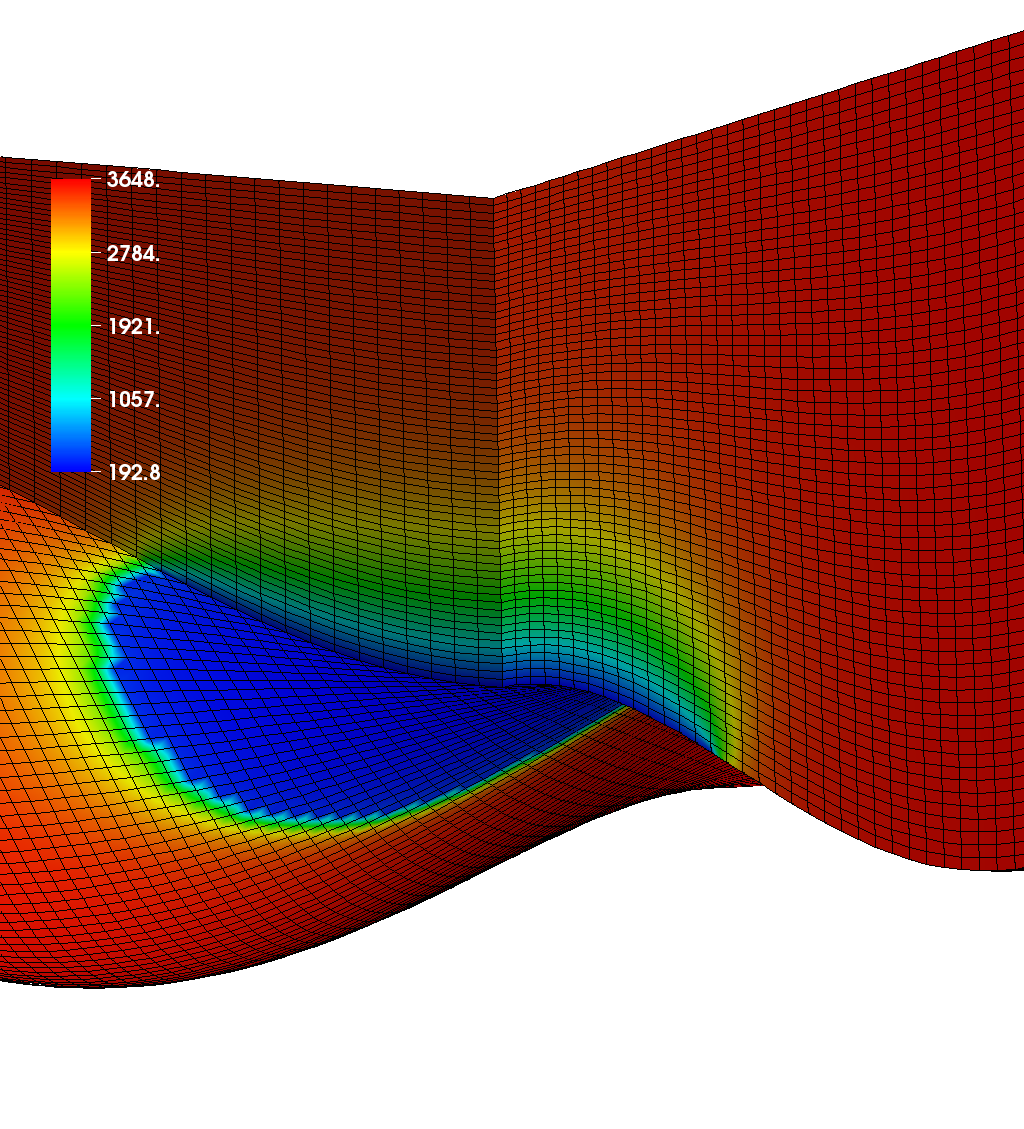
\includegraphics[width=1.2\textwidth]{figures/THI/x-5km-m8p5l5-clip}
}


\begin{frame}{Some Multigrid Options}
  \begin{itemize}
  \item \code{-dmmg\_grid\_sequencce}: [FALSE] \\
    Solve nonlinear problems on coarse grids to get initial guess
  \item \code{-pc\_mg\_galerkin}: [FALSE] \\
    Use Galerkin process to compute coarser operators
  \item \code{-pc\_mg\_type}: [FULL] \\
    (choose one of) MULTIPLICATIVE ADDITIVE FULL KASKADE
  \item \code{-mg\_coarse\_\{ksp,pc\}\_*} \\
    control the coarse-level solver
  \item \code{-mg\_levels\_\{ksp,pc\}\_*} \\
    control the smoothers on levels
  \item \code{-mg\_levels\_3\_\{ksp,pc\}\_*} \\
    control the smoother on specific level
  \item These also work with ML's algebraic multigrid.
  \end{itemize}
\end{frame}

\begin{frame}{What is this doing?}
\begin{itemize}
\item
\begin{alltt}\footnotesize
mpiexec -n 4 ./ex48
-M 16
-P 2
-da\_refine\_hierarchy\_x 1,8,8 \\
-da\_refine\_hierarchy\_y 2,1,1
-da\_refine\_hierarchy\_z 2,1,1 \\
-dmmg\_grid\_sequence 1
-dmmg\_view
-log\_summary \\
-ksp\_converged\_reason
-ksp\_gmres\_modifiedgramschmidt \\
-ksp\_monitor
-ksp\_rtol 1e-2 \\
-pc\_mg\_type multiplicative \\
-mg\_coarse\_pc\_type lu
-mg\_levels\_0\_pc\_type lu \\
-mg\_coarse\_pc\_factor\_mat\_solver\_package mumps \\
-mg\_levels\_0\_pc\_factor\_mat\_solver\_package mumps \\
-mg\_levels\_1\_sub\_pc\_type cholesky \\
-snes\_converged\_reason
-snes\_monitor
-snes\_stol 1e-12 \\
-thi\_L 80e3
-thi\_alpha 0.05
-thi\_friction\_m 0.3 \\
-thi\_hom x
-thi\_nlevels 4
\end{alltt}
\item What happens if you remove \code{-dmmg\_grid\_sequence}?
\item What about solving with block Jacobi, ASM, or algebraic multigrid?
\end{itemize}
\end{frame}

\subsection{Driven cavity}
\begin{frame}{SNES Example}
\framesubtitle{Driven Cavity}
\hbox{
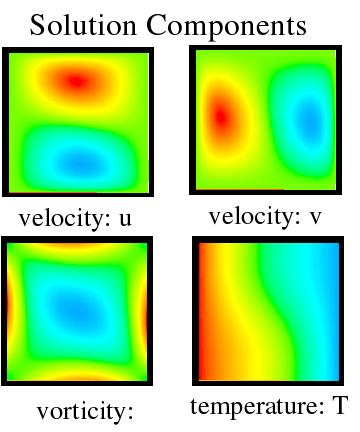
\includegraphics[width=.4\textwidth]{figures/SNES/DrivenCavitySolution}
\vbox{
\begin{itemize}
  \item Velocity-vorticity formulation
  \item Flow driven by lid and/or bouyancy
  \item Logically regular grid
  \begin{itemize}
    \item Parallelized with {\kb DMDA}
  \end{itemize}
  \item Finite difference discretization
  \item Authored by David Keyes
\end{itemize}
}
}
\code{src/snes/examples/tutorials/ex19.c}
\end{frame}

\begin{frame}[fragile]{SNES Example}
\framesubtitle{Driven Cavity Application Context}
\begin{minted}{c}
/* Collocated at each node */
typedef struct {
  PetscScalar u,v,omega,temp;
} Field;

typedef struct {
       /* physical parameters */
   PassiveReal lidvelocity,prandtl,grashof;
       /* color plots of the solution */
   PetscTruth  draw_contours;
} AppCtx;
\end{minted}
\end{frame}

\begin{frame}[fragile]{SNES Example}
\begin{minted}[fontsize=\footnotesize]{c}
DrivenCavityFunction(SNES snes, Vec X, Vec F, void *ptr) {
  AppCtx        *user = (AppCtx *) ptr;
  /* local starting and ending grid points */
  PetscInt       istart, iend, jstart, jend;
  PetscScalar    *f;             /* local vector data */
  PetscReal      grashof = user->grashof;  
  PetscReal      prandtl = user->prandtl;
  PetscErrorCode ierr;

  /* Code to communicate nonlocal ghost point data */
  VecGetArray(F, &f);

  /* Loop over local part and assemble into f[idxloc] */
  /* .... */

  VecRestoreArray(F, &f);
  return 0;
}
\end{minted}
\end{frame}

\begin{frame}[fragile]{SNES Example with local evaluation}
\begin{minted}[fontsize=\footnotesize]{c}
PetscErrorCode DrivenCavityFuncLocal(DMDALocalInfo *info,
                    Field **x,Field **f,void *ctx) {
  /* Handle boundaries ... */
  /* Compute over the interior points */
  for(j = info->ys; j < info->ys+info->ym; j++) {
    for(i = info->xs; i < info->xs+info->xm; i++) {
      /* convective coefficients for upwinding ... */
      /* U velocity */
      u          = x[j][i].u;
      uxx        = (2.0*u - x[j][i-1].u - x[j][i+1].u)*hydhx;
      uyy        = (2.0*u - x[j-1][i].u - x[j+1][i].u)*hxdhy;
      f[j][i].u  = uxx + uyy - .5*(x[j+1][i].omega-x[j-1][i].omega)*hx;
      /* V velocity, Omega ... */
      /* Temperature */
      u             = x[j][i].temp;
      uxx           = (2.0*u - x[j][i-1].temp - x[j][i+1].temp)*hydhx;
      uyy           = (2.0*u - x[j-1][i].temp - x[j+1][i].temp)*hxdhy;
      f[j][i].temp =  uxx + uyy + prandtl
        * (  (vxp*(u - x[j][i-1].temp) + vxm*(x[j][i+1].temp - u)) * hy
           + (vyp*(u - x[j-1][i].temp) + vym*(x[j+1][i].temp - u)) * hx);

}}}
\end{minted}

\begin{center}\small
\$PETSC\_DIR/src/snes/examples/tutorials/ex19.c
\end{center}
\end{frame}


\begin{frame}{Running the driven cavity}
  \begin{itemize}
  \item \code{./ex19 -lidvelocity 100 -grashof 1e2 -da\_grid\_x 16 -da\_grid\_y 16 -snes\_monitor -dmmg\_view -nlevels 3}
  \item \code{./ex19 -lidvelocity 100 -grashof 1e4 -da\_grid\_x 16 -da\_grid\_y 16 -snes\_monitor -dmmg\_view -nlevels 3}
  \item \code{./ex19 -lidvelocity 100 -grashof 1e5 -da\_grid\_x 16 -da\_grid\_y 16 -snes\_monitor -dmmg\_view -nlevels 3}
  \item<2-> Uh oh, we have convergence problems
  \item<2-> Run with \code{-snes\_monitor\_convergence}
  \item<2-> Does \code{-dmmg\_grid\_sequence} help? 
  \end{itemize}
\end{frame}

\begin{frame}{Why isn't SNES converging?}
  \begin{itemize}
  \item The Jacobian is wrong (maybe only in parallel)
    \oneitem{Check with \code{-snes\_type test} and \code{-snes\_mf\_operator -pc\_type lu}}
  \item The linear system is not solved accurately enough
    \begin{itemize}
    \item Check with \code{-pc\_type lu}
    \item Check \code{-ksp\_monitor\_true\_residual}, try right preconditioning
    \end{itemize}
  \item The Jacobian is singular with inconsistent right side
    \begin{itemize}
    \item Use \code{MatNullSpace} to inform the \code{KSP} of a known null space
    \item Use a different Krylov method or preconditioner
    \end{itemize}
  \item The nonlinearity is just really strong
    \begin{itemize}
    \item Run with \code{-info} or \code{-snes\_ls\_monitor} (petsc-dev) to see line search
    \item Try using trust region instead of line search \code{-snes\_type tr}
    \item Try grid sequencing if possible
    \item Use a continuation
    \end{itemize}
  \end{itemize}
\end{frame}

\begin{frame}{Globalizing the lid-driven cavity}
  \begin{block}{Pseudotransient continuation continuation ($\Psi tc$)}
    \begin{itemize}
    \item Do linearly implicit backward-Euler steps, driven by
      steady-state residual
    \item Clever way to adjust step sizes to retain quadratic
      convergence it terminal phase
    \end{itemize}
  \end{block}
  \begin{itemize}
  \item Implemented in \code{src/snes/examples/tutorials/ex27.c}
  \item \shell{make runex27}
  \item Make the method linearly implicit: \code{-snes\_max\_it 1}
    \oneitem{Compare required number of linear iterations}
  \item Try increasing \code{-lidvelocity}, \code{-grashof}, and problem size
  \item Coffey, Kelley, and Keyes, \emph{Pseudotransient continuation and differential algebraic equations}, SIAM J. Sci. Comp, 2003.
  \end{itemize}
\end{frame}


\section{Hard problems}
\begin{frame}{Splitting for Multiphysics}
  \begin{equation*}
    \begin{bmatrix}
      A & B \\ C & D
    \end{bmatrix}
    \begin{bmatrix}
      x \\ y
    \end{bmatrix}
    =
    \begin{bmatrix}
      f \\ g
    \end{bmatrix}
  \end{equation*}
  \begin{itemize}\item Relaxation:
    \code{-pc\_fieldsplit\_type [additive,multiplicative,symmetric\_multiplicative]}
    \begin{equation*}
      \begin{bmatrix}
        A & \\  & D
      \end{bmatrix}^{-1} \qquad 
      \begin{bmatrix}
        A & \\ C & D
      \end{bmatrix}^{-1} \qquad
      \begin{bmatrix}
        A & \\  & \bm 1
      \end{bmatrix}^{-1}
      \left(
        \bm 1 -
        \begin{bmatrix}
          A & B \\ & \bm 1
        \end{bmatrix}
        \begin{bmatrix}
          A & \\ C & D
        \end{bmatrix}^{-1}
      \right)
    \end{equation*}
    \begin{itemize}
    \item Gauss-Seidel inspired, works when fields are loosely coupled
    \end{itemize}
  \item Factorization: \code{-pc\_fieldsplit\_type schur}
    \begin{align*}
      \begin{bmatrix}
        A & B \\ & S
      \end{bmatrix}^{-1}
      \begin{bmatrix}
        1 & \\ CA^{-1} & 1
      \end{bmatrix}^{-1}, \qquad
      S = D - C A^{-1} B
    \end{align*}
    \begin{itemize}
    \item robust (exact factorization), can often drop lower block
    \item how to precondition $S$ which is usually dense?
      \begin{itemize}
      \item interpret as differential operators, use approximate commutators
      \end{itemize}
    \end{itemize}
  \end{itemize}
\end{frame}

\begin{frame}{Coupled approach to multiphysics}
  \begin{itemize}
  \item Smooth all components together
    \begin{itemize}
    \item Block SOR is the most popular
    \item Block ILU sometimes more robust (\eg transport/anisotropy)
    \item Vanka field-split smoothers or for saddle-point problems
    \item Distributive relaxation
    \end{itemize}
  \item Scaling between fields is critical
  \item Indefiniteness
    \begin{itemize}
    \item Make smoothers and interpolants respect inf-sup condition
    \item Difficult to handle anisotropy
    \item Exotic interpolants for Helmholtz
    \end{itemize}
  \item Transport
    \begin{itemize}
    \item Define smoother in terms of first-order upwind discretization ($h$-ellipticity)
    \item Evaluate residuals using high-order discretization
    \item Use Schur field-split: ``parabolize'' at top level or for smoother on levels
    \end{itemize}
  \item Multigrid inside field-split or field-split inside multigrid
  \item Open research area, hard to write modular software
  \end{itemize}
\end{frame}

%\begin{frame}{Anisotropy and Heterogeneity}
  \begin{itemize}
  \item Anisotropy
    \begin{itemize}
    \item Semi-coarsening
    \item Line smoothers
    \item Order unknowns so that incomplete factorization ``includes'' a
      line smoother
    \end{itemize}
  \item Heterogeneity
    \begin{itemize}
    \item Make coarse grids align
    \item Strong smoothers
    \item Energy-minimizing interpolants
    \end{itemize}
  \end{itemize}
\end{frame}

\begin{frame}[shrink=10]{``Physics-based'' preconditioners (semi-implicit method)}
  \begin{block}{Shallow water with stiff gravity wave}
    $h$ is hydrostatic pressure, $u$ is velocity, $\sqrt{gh}$ is fast wave speed
    \begin{gather*}
      h_t - (uh)_x = 0 \\
      (uh)_t + (u^2h + \half gh^2)_x = 0
    \end{gather*}
  \end{block}
  \vspace{-3em}
  \begin{block}{Semi-implicit method}
    Suppress spatial discretization, discretize in time, implicitly for the terms contributing to the gravity wave
    \begin{gather*}
      \frac{h^{n+1} - h^n}{\Delta t} + (uh)_x^{n+1} = 0 \\
      \frac{(uh)^{n+1} - (uh)^{n}}{\Delta t} + (u^2h)_x^{n} + g(h^n h^{n+1})_x = 0
    \end{gather*}

    Rearrange, eliminating $(uh)^{n+1}$
    \[ \frac{h^{n+1} - h^n}{\Delta t} - \Delta t(gh^n h_x^{n+1})_x = -S_x^n \]
  \end{block}
\end{frame}

\begin{frame}[shrink=1]{Delta form}
  \begin{itemize}
  \item Preconditioner should work like the Newton step: $-F(x) \mapsto \delta x$
  \item Recast semi-implicit method in delta form
    \[ \frac{\delta h}{\Delta t} + (\delta uh)_x = -F_0, \quad \frac{\delta uh}{\Delta t} + g h^n (\delta h)_x = -F_1,
    \quad \widehat{J} =
    \begin{pmatrix}
      \frac{1}{\Delta t} & \div \\
      g h^n \nabla & \frac{1}{\Delta t}
    \end{pmatrix}
    \]
  \item Eliminate $\delta uh$
    \[ \frac{\delta h}{\Delta t} - \Delta t(gh^n (\delta h)_x)_x = -F_0 + (\Delta t F_1)_x,
    \quad S \sim \frac{1}{\Delta t} - g \Delta t \div h^n \nabla
    \]
  \item Solve for $\delta h$, then evaluate
    \[ \delta uh = - \Delta t \big[ gh^n (\delta h)_x - F_1 \big] \]
  \item Fully implicit solver
    \begin{itemize}
    \item Is nonlinearly consistent (no splitting error), can be high-order in time
    \item Uses existing code when a semi-implicit method has been implemented
    \item Allows efficient bifurcation analysis, steady-state analysis
    \end{itemize}
  \end{itemize}
\end{frame}


\section{Recent developments in PETSc}
\subsection{Improved multiphysics support}
\begin{frame}{Multiphysics problems}
  \begin{block}{Examples}
    \begin{itemize}
    \item Saddle-point problems (\eg incompressibility, contact)
    \item Stiff waves (\eg low-Mach combustion)
    \item Mixed type (\eg radiation hydrodynamics, ALE free-surface flows)
    \item Multi-domain problems (\eg fluid-structure interaction)
    \item Full space PDE-constrained optimization
    \end{itemize}
  \end{block}
  \begin{block}{Software/algorithmic considerations}
    \begin{itemize}
    \item Separate groups develop different ``physics'' components
    \item Do not know a priori which methods will have good algorithmic properties
    \item Achieving high throughput is more complicated
    \item Multiple time and/or spatial scales
      \begin{itemize}
      \item Splitting methods are delicate, often not in asymptotic regime
      \item Strongest nonlinearities usually non-stiff: prefer explicit for TVD limiters/shocks
      \end{itemize}
    \end{itemize}
  \end{block}
\end{frame}

\begin{frame}{The Great Solver Schism: Monolithic or Split?}
  \begin{columns}
    \begin{column}{0.5\textwidth}
      \begin{block}{Monolithic}
        \begin{itemize}
        \item Direct solvers
        \item Coupled Schwarz
        \item Coupled Neumann-Neumann \\
          (need unassembled matrices)
        \item Coupled multigrid
        \item[X] Need to understand local spectral and compatibility properties of the coupled system
        \end{itemize}
      \end{block}
    \end{column}
    \begin{column}{0.5\textwidth}
      \begin{block}{Split}
        \begin{itemize}
        \item Physics-split Schwarz \\
          (based on relaxation)
        \item Physics-split Schur \\
          (based on factorization)
          \begin{itemize}
          \item  approximate commutators \\
            SIMPLE, PCD, LSC
          \item segregated smoothers
          \item Augmented Lagrangian
          \item ``parabolization'' for stiff waves
          \end{itemize}
        \item[X] Need to understand global coupling strengths
        \end{itemize}
      \end{block}
    \end{column}
  \end{columns}
  \begin{itemize}
  \item Preferred data structures depend on which method is used.
  \item Interplay with geometric multigrid.
  \end{itemize}
\end{frame}

\begin{frame}{Multi-physics coupling in PETSc}
  \begin{columns}
    \begin{column}{0.5\textwidth}
      \tikzstyle{cloud} = [draw, ellipse,fill=red!20, node distance=3cm, minimum height=2em]
      \tikzstyle{block} = [rectangle, draw, fill=blue!20, text width=5em, text centered, rounded corners, minimum height=2em]
      \begin{tikzpicture}
        \node [cloud] (momentum) {Momentum};
        \node [cloud, right of=momentum] (pressure) {Pressure};
        \node<2-> [block, opacity=0.5, fit=(momentum)(pressure), text opacity=0.8] (stokes) {Stokes};
        \node<3-> [cloud, below=2em of momentum] (energy) {Energy};
        \node<3-> [cloud, below=2em of pressure] (geometry) {Geometry};
        \node<4-> [block, opacity=0.4, fit=(stokes)(momentum)(pressure)(energy)(geometry), text opacity=0.8, text height=4em] (ice) {Ice};
        \node<5-> [block, below=2em of ice, minimum width=16em] (bl) {{Boundary \nolinebreak Layer}};
        \node<5-> [block, below=2em of bl, minimum width=16em] (ocean) {Ocean};
        % ]
      \end{tikzpicture}
    \end{column}
    \begin{column}{0.5\textwidth}
      \begin{itemize}
      \item package each ``physics'' independently
      \item solve single-physics and coupled problems
      \item semi-implicit and fully implicit
      \item reuse residual and Jacobian evaluation unmodified
      \item direct solvers, fieldsplit inside multigrid, multigrid inside fieldsplit without recompilation
      \item use the best possible matrix format for each physics \\ (e.g. symmetric block size 3)
      \item matrix-free anywhere
      \item multiple levels of nesting
      \end{itemize}
    \end{column}
  \end{columns}
\end{frame}

\begin{frame}
  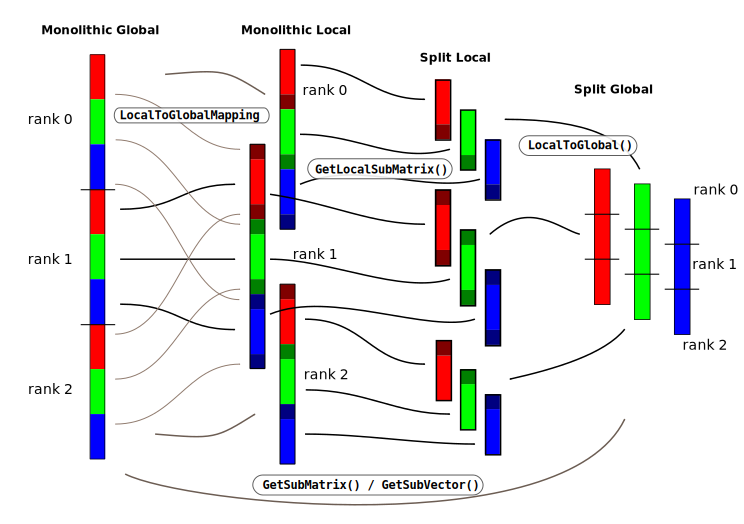
\includegraphics[width=\textwidth]{figures/PETSc/LocalSpaces} \\[-.5em]
  Work in Split Local space, matrix data structures reside in any space.
\end{frame}

\begin{frame}[fragile]{Multiphysics Assembly Code: Residuals}
\begin{minted}[fontsize=\footnotesize]{c}
FormFunction_Coupled(SNES snes,Vec X,Vec F,void *ctx) {
  struct UserCtx *user = ctx;
  // ...
  SNESGetDM(snes,&pack);
  DMCompositeGetEntries(pack,&dau,&dak);
  DMDAGetLocalInfo(dau,&infou);
  DMDAGetLocalInfo(dak,&infok);
  DMCompositeScatter(pack,X,Uloc,Kloc);
  DMDAVecGetArray(dau,Uloc,&u);
  DMDAVecGetArray(dak,Kloc,&k);
  DMCompositeGetAccess(pack,F,&Fu,&Fk);
  DMDAVecGetArray(dau,Fu,&fu);
  DMDAVecGetArray(dak,Fk,&fk);
  FormFunctionLocal_U(user,&infou,u,k,fu); // u residual with k given
  FormFunctionLocal_K(user,&infok,u,k,fk); // k residual with u given
  DMDAVecRestoreArray(dau,Fu,&fu);
  // More restores
\end{minted}
\end{frame}

\begin{frame}[fragile]{Multiphysics Assembly Code: Jacobians}
\begin{minted}[fontsize=\footnotesize]{c}
FormJacobian_Coupled(SNES snes,Vec X,Mat J,Mat B,...) {
  // Access components as for residuals
  MatGetLocalSubMatrix(B,is[0],is[0],&Buu);
  MatGetLocalSubMatrix(B,is[0],is[1],&Buk);
  MatGetLocalSubMatrix(B,is[1],is[0],&Bku);
  MatGetLocalSubMatrix(B,is[1],is[1],&Bkk);
  FormJacobianLocal_U(user,&infou,u,k,Buu);         // single physics
  FormJacobianLocal_UK(user,&infou,&infok,u,k,Buk); // coupling
  FormJacobianLocal_KU(user,&infou,&infok,u,k,Bku); // coupling
  FormJacobianLocal_K(user,&infok,u,k,Bkk);         // single physics
  MatRestoreLocalSubMatrix(B,is[0],is[0],&Buu);
  // More restores
\end{minted}
\begin{itemize}
\item Assembly code is independent of matrix format
\item Single-physics code is used unmodified for coupled problem
\item No-copy fieldsplit: \verb|-pack_dm_mat_type nest -pc_type fieldsplit|
\item Coupled direct solve: \\
  {\scriptsize \verb|-pack_dm_mat_type aij -pc_type lu -pc_factor_mat_solver_package mumps|}
\end{itemize}
\end{frame}

\begin{frame}
  \alert{\texttt{MatGetLocalSubMatrix(Mat A,IS rows,IS cols,Mat *B);}}
  \begin{itemize}
  \item Primarily for assembly
    \begin{itemize}
    \item \texttt{B} is not guaranteed to implement \texttt{MatMult}
    \item The communicator for \texttt{B} is not specified, \\
      only safe to use non-collective ops (unless you check)
    \end{itemize}
  \item \texttt{IS} represents an index set, includes a block size and communicator
  \item \texttt{MatSetValuesBlockedLocal()} is implemented
  \item MatNest returns nested submatrix, no-copy
  \item No-copy for Neumann-Neumann formats \\ (unassembled across procs, e.g. BDDC, FETI-DP)
  \item Most other matrices return a lightweight proxy \texttt{Mat}
    \begin{itemize}
    \item \texttt{COMM\_SELF}
    \item Values not copied, does not implement \texttt{MatMult}
    \item Translates indices to the language of the parent matrix
    \item Multiple levels of nesting are flattened
    \end{itemize}
  \end{itemize}
\end{frame}

\subsection{Variational inequalities}
\begin{frame}{Variational Inequalities}
  \begin{itemize}
  \item Supports inequality and box constraints on solution variables.
  \item Solution methods
    \begin{itemize}
    \item Semismooth Newton
      \begin{itemize}
      \item reformulate problem as a non-smooth system, Newton on subdifferential
      \item Newton step solves diagonally perturbed systems
      \end{itemize}
    \item Active set
      \begin{itemize}
      \item similar linear algebra to solving PDE
      \item sometimes slower convergence or ``bouncing''
      \end{itemize}
    \end{itemize}
  \item composes with multigrid and field-split
  \item demonstrated optimality for phase-field problems with millions of degrees of freedom
  \end{itemize}
\end{frame}



\begin{frame}{References}
  \begin{itemize}
  \item Knoll and Keyes, \emph{Jacobian-free Newton-Krylov methods: a survey of approaches and applications}, JCP, 2004.
  \item Elman et. al., \emph{A Taxonomy and Comparison of Parallel Block Multi-Level Preconditioners for the Incompressible Navier-Stokes Equations}, JCP, 2008.
  \item Wan, Chan, and Smith, \emph{An Energy-minimizing Interpolation for Robust Multigrid Methods}, SIAM J. Sci. Comp, 2000.
  \item Gropp, Kaushik, Keyes, Smith, \emph{Performance Modeling and Tuning of an Unstructured Mesh CFD Application}, Supercomputing, 2000.
  \item Gropp, \emph{Exploiting Existing Software in Libraries: Successes, Failures, and Reasons Why}, OO methods for interoperable scientific and engineering computing, 1999.
  \item ICiS Multiphysics workshop report:  IJHPCA 27(1), Feb 2013, http://dx.doi.org/10.1177/1094342012468181 \\
    \url{http://www.ipd.anl.gov/anlpubs/2012/01/72183.pdf}
  \end{itemize}
\end{frame}

\end{document}
